% LaTeX: More Than Just Academic Papers and Journals
%
% Copyright Lim Lian Tze 2011 (liantze@gmail.com) 
% Beamer presentation slides for a talk at the Malaysian Open Source Conference 
% 2011 (MOSC 2011 http://www.mosc.my/)
%
% http://liantze.penguinattack.org/latextypesetting.html
%
% This work is licensed under a Creative Commons Attribution-NonCommercial-
% ShareAlike 3.0 Unported License (http://creativecommons.org/licenses/by-nc-sa/3.0/).
%

\pdfminorversion=5
\pdfobjcompresslevel=3 
\pdfcompresslevel=9

% Full presentation (with overlays, animated bullet items etc)
\documentclass[xcolor={x11names,svgnames,dvipsnames}]{beamer}

% Transparency mode (no overlays)
%\documentclass[xcolor={x11names,svgnames,dvipsnames},trans]{beamer}

% 4-up handout mode
%\documentclass[xcolor={x11names,svgnames,dvipsnames},handout]{beamer}

\usepackage{pgfpages}
\usepackage[british]{babel}
\usepackage{etex}

%% Glossy pretty look for the presentation and transparency (w/o overlays and animations) versions!
\mode<beamer|trans>{
\useoutertheme[glossy]{wuerzburg}
\useinnertheme[shadow,outline]{chamfered}
\usecolortheme{shark}
}
\setbeamertemplate{navigation symbols}{}
\setbeamertemplate{frametitle continuation}[from second][(cont'd)]
\usefonttheme[stillsansseriftext,stillsansserifsmall]{serif}

%% Save up on ink for the 4-up handouts
\mode<handout>{
\useoutertheme{wuerzburg}
\useinnertheme[outline]{chamfered}
\pgfpagesuselayout{4 on 1}[a4paper, landscape, border shrink=10mm]
\pgfpageslogicalpageoptions{1}{border code=\pgfstroke}
\pgfpageslogicalpageoptions{2}{border code=\pgfstroke}
\pgfpageslogicalpageoptions{3}{border code=\pgfstroke}
\pgfpageslogicalpageoptions{4}{border code=\pgfstroke}
}

\mode<presentation>{\AtBeginSection{%
\begin{frame}
\frametitle{Contents}
\tableofcontents[currentsection]
\end{frame}}}

\usepackage{microtype}
\usepackage[utf8]{inputenc}
\usepackage[T1]{fontenc}
\usepackage[osfss]{libertine}
\usepackage[scaled=.77]{beramono}
\usepackage{cmap}

\usepackage{relsize,tabularx}
\usepackage[T1,safe]{tipa}
\usepackage{dtklogos,hologo,textcomp}
\usepackage{multicol,booktabs}
\usepackage{listings}
\lstset{upquote,keepspaces=true,columns=spaceflexible,
basicstyle=\ttfamily\scriptsize,%
breaklines=true,breakindent=0pt,xleftmargin=0pt, xrightmargin=6pt,%
language=[LaTeX]TeX, texcsstyle=*\bfseries\color{Maroon}, commentstyle=\sffamily\itshape\smaller\color{SeaGreen4},
emphstyle=\bfseries\color{RoyalBlue3},escapechar={:},
emphstyle={[2]{\bfseries\color{Sienna2}}},
postbreak=\mbox{{\smaller\color{gray}$\hookrightarrow$}}
}

\usepackage{tikz}
\usetikzlibrary{shapes,arrows,positioning,matrix,chains,backgrounds,fit}

\usepackage{multicol}
\usepackage[version=3]{mhchem}
\usepackage{chemfig}
\usepackage{linguex,qtree}
\let\fg\lingfg
\usepackage{texshade}
\usepackage[detect-all]{siunitx}
\usepackage[siunitx]{circuitikz}
\usepackage{bytefield}
\usepackage{auto-pst-pdf}
\usepackage{pstricks,pst-barcode}
\usepackage{pgfplots}
\usepackage{pgfgantt}
\usepackage[skaknew]{chessboard,skak}
\usepackage{cwpuzzle}
\usepackage{gchords,guitar}
\usepackage{spreadtab}
\usepackage{ccicons}

%\includeonly{intro}
%\includeonly{document}
%\includeonly{intro,domain}


\setlength\fboxsep{0pt}
\SetTracking{encoding=*}{-39}

\author[\textsc{Lim} Lian Tze]{\textsc{Lim} Lian Tze\\[1ex]%
{\small\url{liantze@gmail.com}\\[-.5ex]\url{http://liantze.penguinattack.org/}}\\[.5ex]\ccbyncsa}
\title{\LaTeX: More Than Just Academic Papers and Theses}
%\titlegraphic{\ccbyncsa}
\date[\textsc{mosc} 2011]{Malaysian Open Source Conference 2011}%

% Include QR code of slides URL for presentation-mode only -- so that audience
%  can snap it and download it on the spot
\mode<beamer>{\titlegraphic{\begin{pspicture}\psbarcode[scalex=.75,scaley=.75]{http://liantze.penguinattack.org/latextypesetting.html\#mosc11-slides}{eclevel=L}{qrcode}\end{pspicture}}}

\hypersetup{%
pdfauthor={Lim Lian Tze}, %% the "author" field from above includes garbage code...
pdfkeywords={latex,MOSC2011,general}
}

\begin{document}
\begin{frame}
\maketitle
\end{frame}

\begin{frame}
\frametitle{Contents}
\tableofcontents
\end{frame}

% !TEX root = talk.tex
\section[Introduction]{What are \TeX, \LaTeX\ and Friends?}
\begin{frame}
\frametitle{What are \TeX\ and \LaTeX,\ and Friends?}

\begin{description}
\item<1>[\TeX] 
\begin{itemize}
\item \textsmaller{ASCII} \texttt{TeX}, \textsmaller{\textipa{/tEx/}, \textipa{/tEk/}}
\item A \structure{computer typesetting system} created by Donald Knuth
\item for `the creation of beautiful books'
\end{itemize}


\item<2>[\LaTeX]
\begin{itemize}
\item \textsmaller{ASCII} \texttt{LaTeX}, \textsmaller{\textipa{/"leItEx/}, \textipa{/"leItEk/}, \textipa{/"lA:tEx/}, \textipa{/"lA:tEk/}}
\item A \structure{document preparation system} by Leslie Lamport
	\end{itemize}

\pause

\item<3-4>[Binaries]
	\begin{itemize}
  \item \structure{\hologo{eTeX}}: additional primitives to \hologo{TeX}
	\item \structure{\alert<4>{\hologo{pdfTeX}}}: additional PDF-related primitives
  \item \structure{\XeTeX}: native UTF-8 input; can access system fonts
	\item \structure{\hologo{LuaTeX}}: includes the Lua scripting engine
\end{itemize}
\item <5>[Friends]
\begin{itemize}
\item \structure{\BibTeX}, \structure{\MakeIndex}, \structure{\METAFONT}, \structure{METAPOST},  \ldots
\item \url{http://www.ctan.org/what_is_tex.html}
\end{itemize}
\end{description}
\end{frame}

\begin{frame}
\frametitle{Why?}
\framesubtitle{From \url{http://www.ctan.org/what_is_tex.html}}
\begin{columns}[T]
\begin{column}{.46\textwidth}
\begin{block}{Output Quality}
\begin{itemize}
\item It has the best output.
\item It knows typesetting.
\end{itemize}
\end{block}

\begin{block}{Superior Engineering}
\begin{itemize}
\item It's fast.
\item It's stable.
\item It's not rigid (extensible).
\item Plain text input.
\item Many output types.
\end{itemize}
\end{block}
\end{column}

\begin{column}{.46\textwidth}
\begin{block}{Freedom}
\begin{itemize}
\item It's free.
\item It runs anywhere.
\end{itemize}
\end{block}

\begin{block}{Popularity}
\begin{itemize}
\item It's the standard (in academia and science).
\end{itemize}
\end{block}
\end{column}
\end{columns}
\end{frame}

\begin{frame}
\frametitle{Where Would I Want to Use \hologo{LaTeX}?}
\begin{itemize}
\item Documents with complex structures
\item Lots of mathematics \pause(or other specific needs)\pause
\item When publishers \alert{require} them
\pause
\item Batch processing
\pause
\item Back-end of other applications
\end{itemize}
\end{frame}

\begin{frame}
\frametitle{How Do I Use It?}
\begin{enumerate}
\item<+-> Write a plain text \hologo{LaTeX} file (\texttt{.tex})
\item<+-> Run it through \texttt{pdflatex} or \texttt{xelatex} $\rightarrow$ \textsmaller{PDF} output\\
\textsmaller{(or \texttt{latex + dvips + ps2pdf} for \textsmaller{DVI} + \textsmaller{PS} + \textsmaller{PDF})}
\item<+-> Run \texttt{bibtex} and/or \texttt{makeindex} to process bibliographies, indices
\item<+-> Re-run \texttt{pdflatex} to resolve references and pointers
\end{enumerate}
\end{frame}

\begin{frame}[fragile]
\frametitle{Example \texttt{.tex} File}

\begin{columns}[T]
\begin{column}{.47\textwidth}
\begin{beamerboxesrounded}[width=\linewidth]{}
\vskip-1.2em
\begin{lstlisting}[moretexcs={maketitle,tableofcontents,subsection},
emph={document,abstract},
basicstyle={\ttfamily\footnotesize\lsstyle},lineskip=-2pt]
\documentclass[a4paper,11pt]{article}
\author{Lim Lian Tze}
\title{An Introductory Paper}
\date{\today}
:\onslide<1-3>{{\bfseries\color{Maroon}\textbackslash usepackage}[\textcolor{Sienna2}{\bfseries english}]\{\textcolor{RoyalBlue3}{\bfseries babel}\}}%
\onslide<4|trans:0|handout:0>{\llap{{\bfseries\color{Maroon}\textbackslash usepackage}[\textcolor{Sienna2}{\bfseries ngerman}]\{\textcolor{RoyalBlue3}{\bfseries babel}\}}}%
\onslide<5|trans:0|handout:0>{\llap{{\bfseries\color{Maroon}\textbackslash usepackage}[\textcolor{Sienna2}{\bfseries bahasam}]\{\textcolor{RoyalBlue3}{\bfseries babel}\}}}:

\begin{document}
\maketitle
\tableofcontents

\begin{abstract}
This paper introduces\ldots
\end{abstract}

\section{Introduction}
We consider\ldots

\section{State of the Art}
We look at\ldots

\subsection{Document Formats}
There are many\ldots
\end{document}
\end{lstlisting}
\vspace*{-1.2em}
\end{beamerboxesrounded}
\end{column}

\begin{column}{.46\textwidth}
\hfill\uncover<3>{\fcolorbox{black}{white}{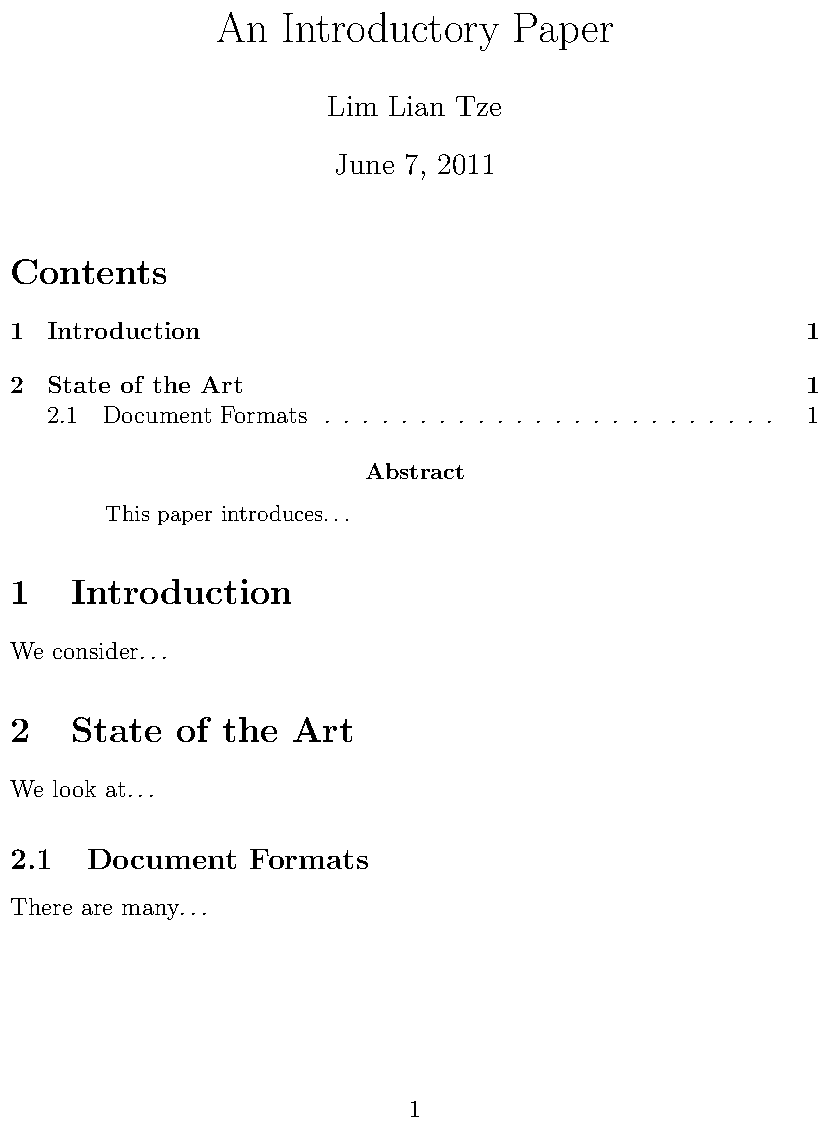
\includegraphics[width=.95\linewidth]{examples/first-en}}}%
\uncover<4|trans:0|handout:0>{\llap{\fcolorbox{black}{white}{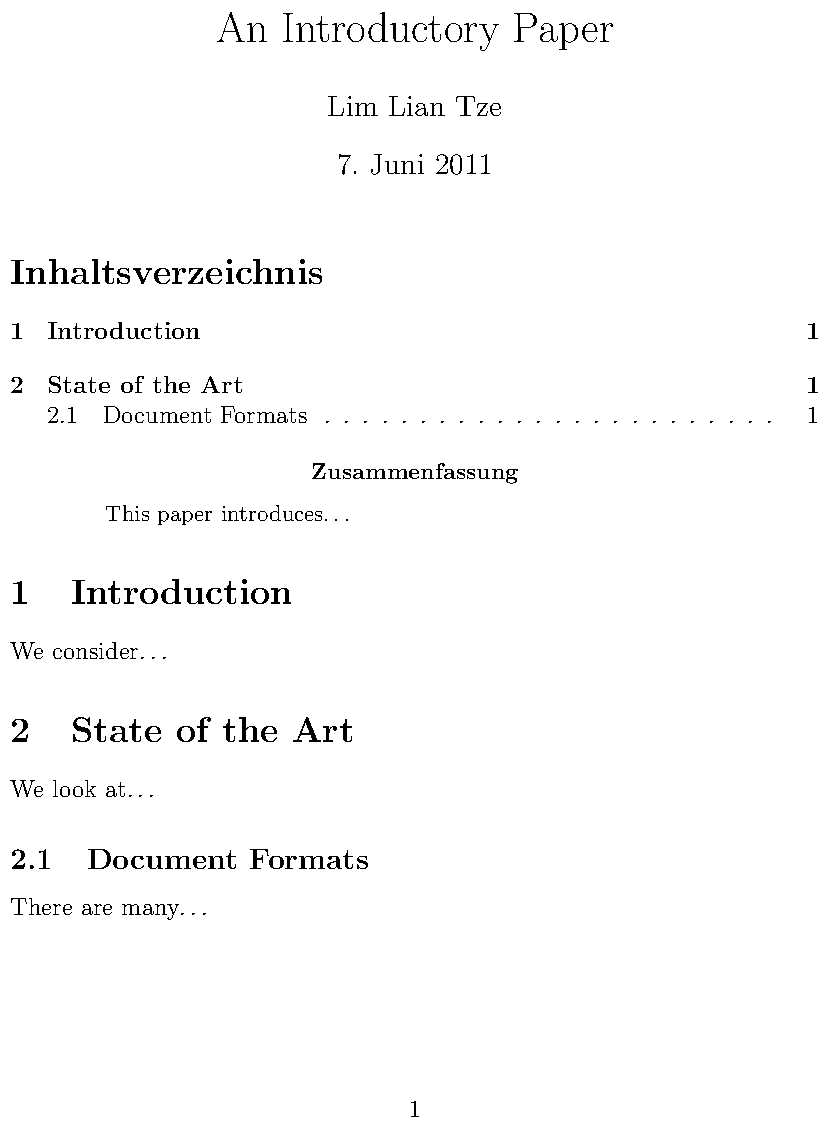
\includegraphics[width=.95\linewidth]{examples/first-de}}}}%
\uncover<5|trans:0|handout:0>{\llap{\fcolorbox{black}{white}{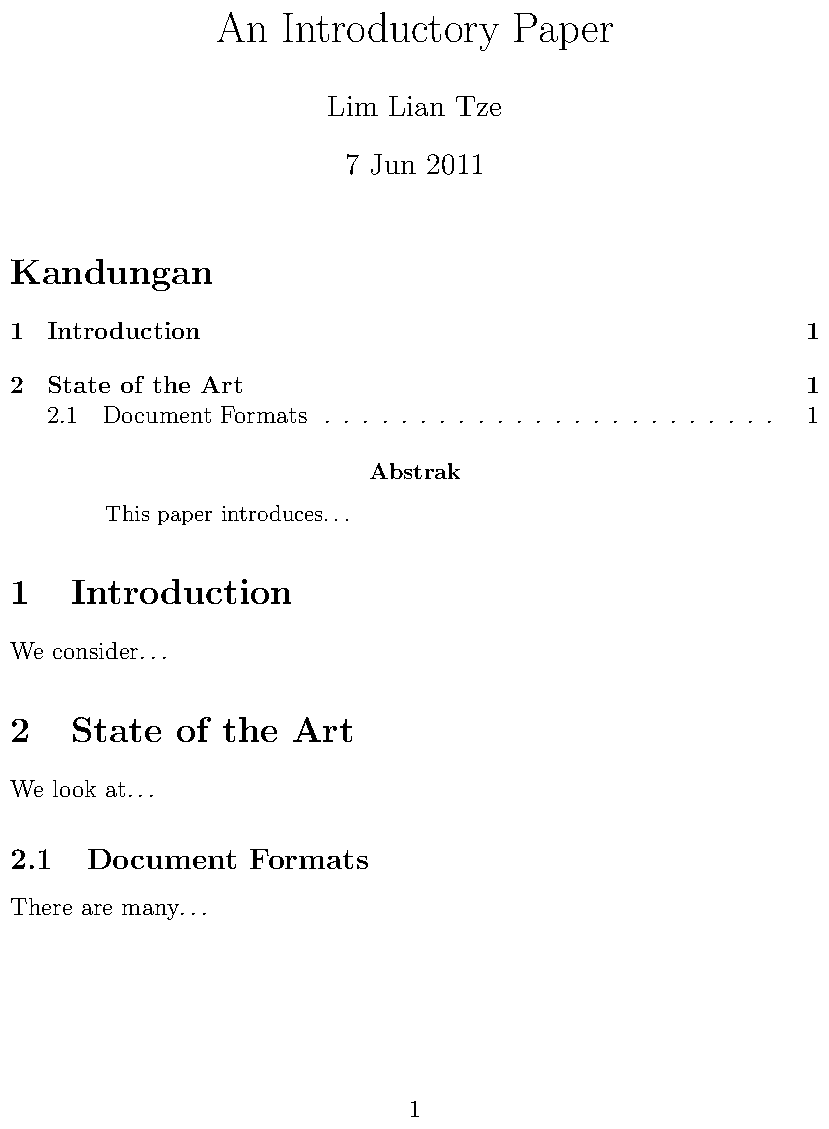
\includegraphics[width=.95\linewidth]{examples/first-ms}}}}
\end{column}
\end{columns}

\uncover<2->{\tikz[remember picture,overlay]\node[single arrow,fill=DarkSeaGreen,font=\ttfamily\bfseries,xshift=-1em] at (current page.center) {pdflatex};}

\end{frame}

\begin{frame}
\frametitle{Where Do I Get It?}
\begin{description}
\setlength\labelwidth{8.5em}
\setlength\itemindent{3em}
\item[Windows] \MikTeX, \TeX Live
\item[Un*x, \textsmaller{GNU}/Linux] \TeX Live
\item[Mac OS X] Mac\TeX\ (based on \TeX Live)
\item[Installation] Use your OS' package manager\\\hspace{\itemindent}(or download manually)
\pause
\item[Editors] vi, emacs, Texmaker, TeXworks, \ldots
\pause
\item[\hologo{LaTeX} Packages] Use \MikTeX\ or \TeX Live's package manager
\pause
\item[Documentation] 
{\small (\TeX Live)} \texttt{\$ texdoc <package name>}\\
\hspace{\itemindent}{\small (\MikTeX)} \texttt{\$ mthelp <package name>}
\end{description}
\end{frame}

\begin{frame}
\frametitle{Easy to Learn, Hard to Master}
\begin{itemize}
\item<+-> Customising may not be straightforward (vs word processors)
\item<+-> Intentionally so: Style guidelines should be followed strictly
\begin{itemize}
\item Publisher/organisation provides \structure{\texttt{document class}} or \structure{\texttt{style}} files
\item Use these to take care of formatting and styling, focus on the \structure{content}
\end{itemize}
\item<+-> Fair enough. \\But where do I learn all the stuff the \TeX nicians and \TeX perts do?
\item<+-> (There \emph{is} a learning curve)
\end{itemize}
\end{frame}

\begin{frame}[label=help]
\frametitle{Getting Help}
\begin{itemize}
\item<+-> Many free tutorials and e-books on the Web (beware of obsolete ones!)
\begin{itemize}
\item \structure{Getting to Grips with \hologo{LaTeX}.}\; Andy Roberts. \url{http://www.andy-roberts.net/misc/latex/}
\item \structure{\hologo{LaTeX}: Beautiful Typesetting.}\; Lim Lian Tze. \url{http://liantze.penguinattack.org/latextypesetting.html}
\item \structure{\hologo{LaTeX} and Friends.}\; M.R.C.\ van Dongen. \url{http://csweb.ucc.ie/~dongen/LaTeX-and-Friends.pdf}
\item \structure{The \hologo{LaTeX} WikiBook.}\; \url{http://en.wikibooks.org/wiki/LaTeX}
\end{itemize}

\item<+-> Questions?
\begin{itemize}
\item \hologo{TeX} \textsmaller{FAQ}.\;  \url{http://www.tex.ac.uk/cgi-bin/texfaq2html}
\item \hologo{TeX}.SX.\; \url{http://tex.stackexchange.com/}
\item \texttt{comp.text.tex} usenet group
\item Malaysian \hologo{LaTeX} User Group.\; \url{http://latex-my.blogspot.com/}
\end{itemize}

\item<3-> Arrange for training
\end{itemize}
\end{frame}


\begin{frame}
\centering\Huge
So, What Can \hologo{LaTeX} Do?
\par
\end{frame}
% !TEX root=talk.tex

\section{Document Types}

\begin{frame}[fragile,allowframebreaks]
\frametitle{Basic Types}
\begin{columns}
\begin{column}{.35\textwidth}
\begin{beamerboxesrounded}[width=\linewidth]{Books}
\begin{lstlisting}[moretexcs={chapter,subsection,maketitle}, basicstyle={\ttfamily}, emph={book}]
\documentclass{book}
\author{...}
\title{...}

\begin{document}
\maketitle
\chapter{...}
\section{...}
...
\subsection{...}
\end{document}
\end{lstlisting}
\end{beamerboxesrounded}
\end{column}
\begin{column}{.58\textwidth}
\centering
\fcolorbox{black}{white}{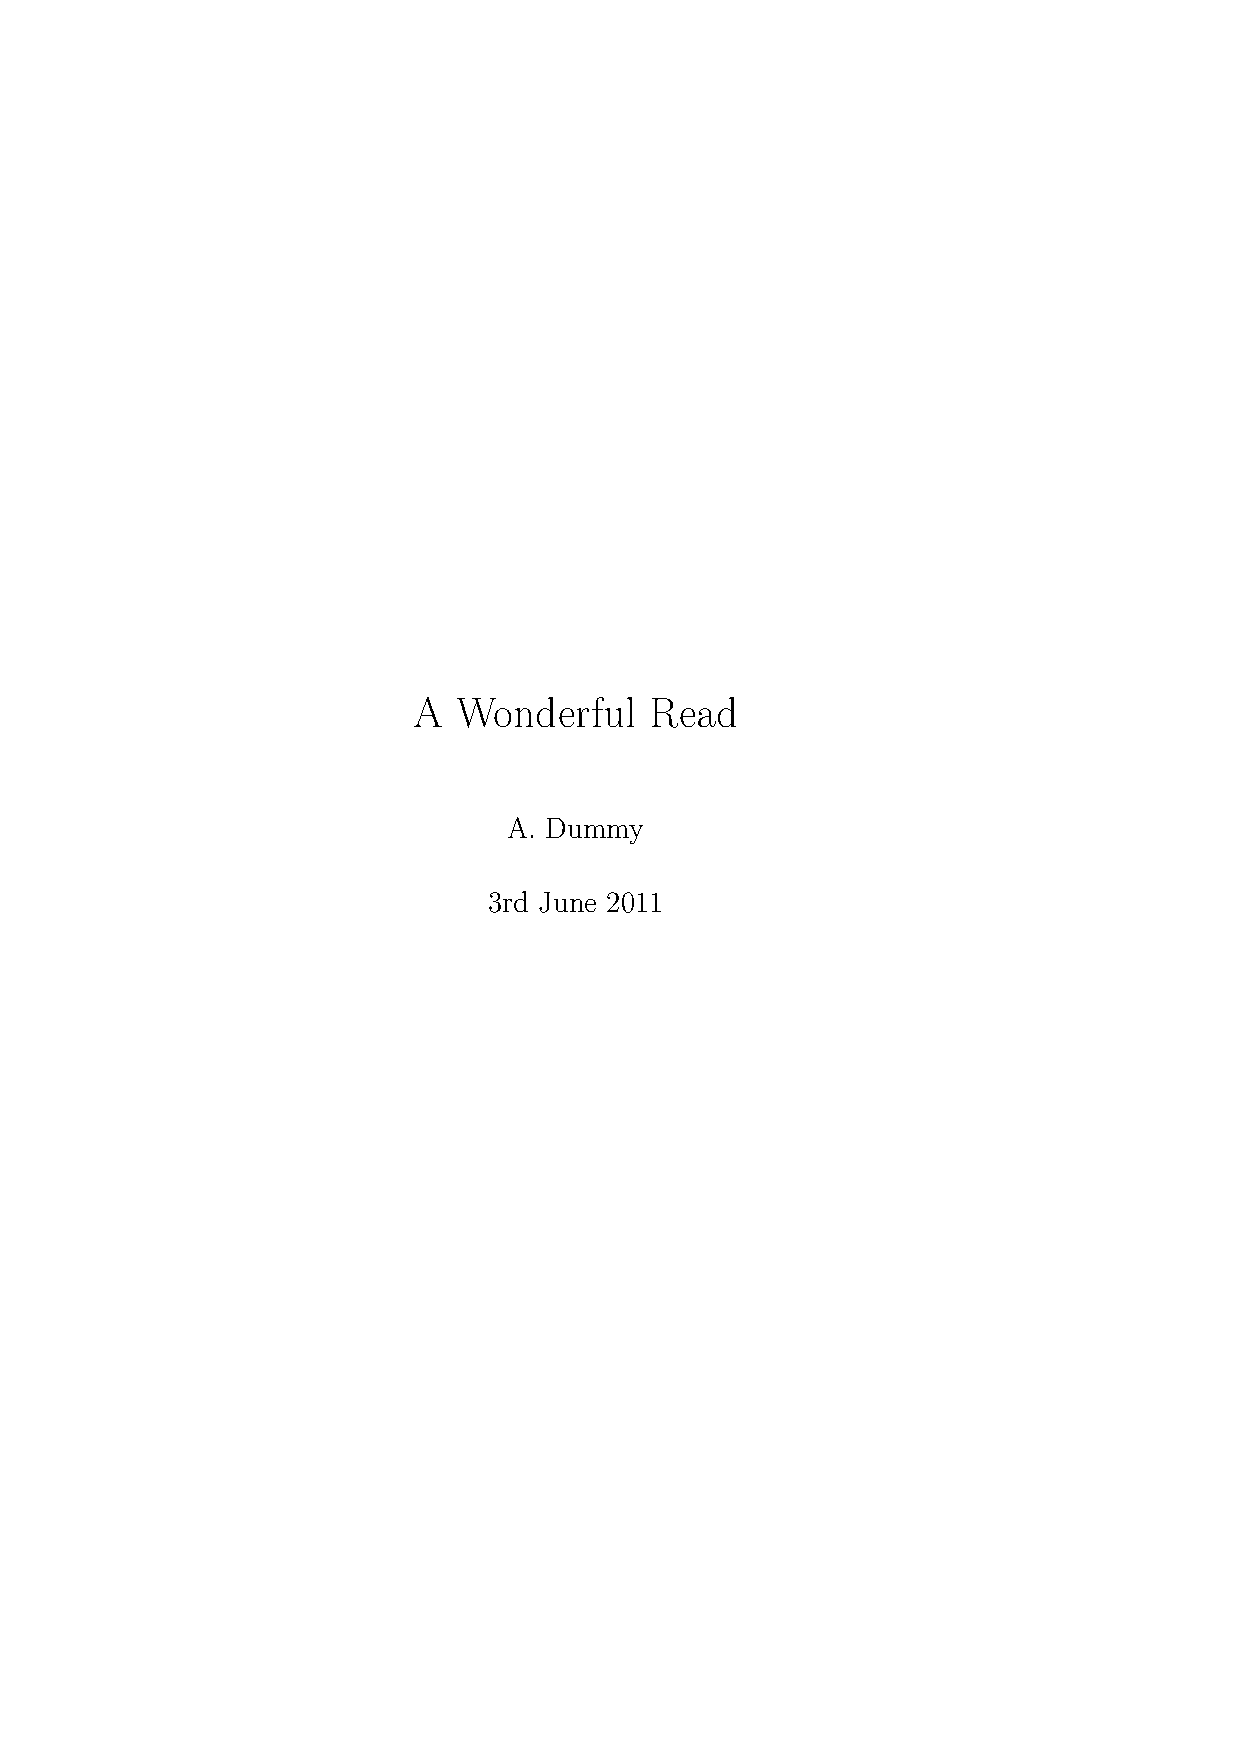
\includegraphics[width=.4\linewidth,page=1]{examples/basicbook}}
\fcolorbox{black}{white}{\includegraphics[width=.4\linewidth,page=3]{examples/basicbook}}
\fcolorbox{black}{white}{\includegraphics[width=.4\linewidth,page=4]{examples/basicbook}}
\fcolorbox{black}{white}{\includegraphics[width=.4\linewidth,page=5]{examples/basicbook}}
\end{column}
\end{columns}

\begin{columns}
\begin{column}{.4\textwidth}
\begin{beamerboxesrounded}[width=\linewidth]{Articles}
\begin{lstlisting}[moretexcs={chapter,subsection,maketitle}, basicstyle={\ttfamily}, emph={article}]
\documentclass{article}
\author{...}
\title{...}

\begin{document}
\maketitle
\section{...}
...
\subsection{...}
\end{document}
\end{lstlisting}
\end{beamerboxesrounded}
\end{column}
\begin{column}{.58\textwidth}
\centering
\fcolorbox{black}{white}{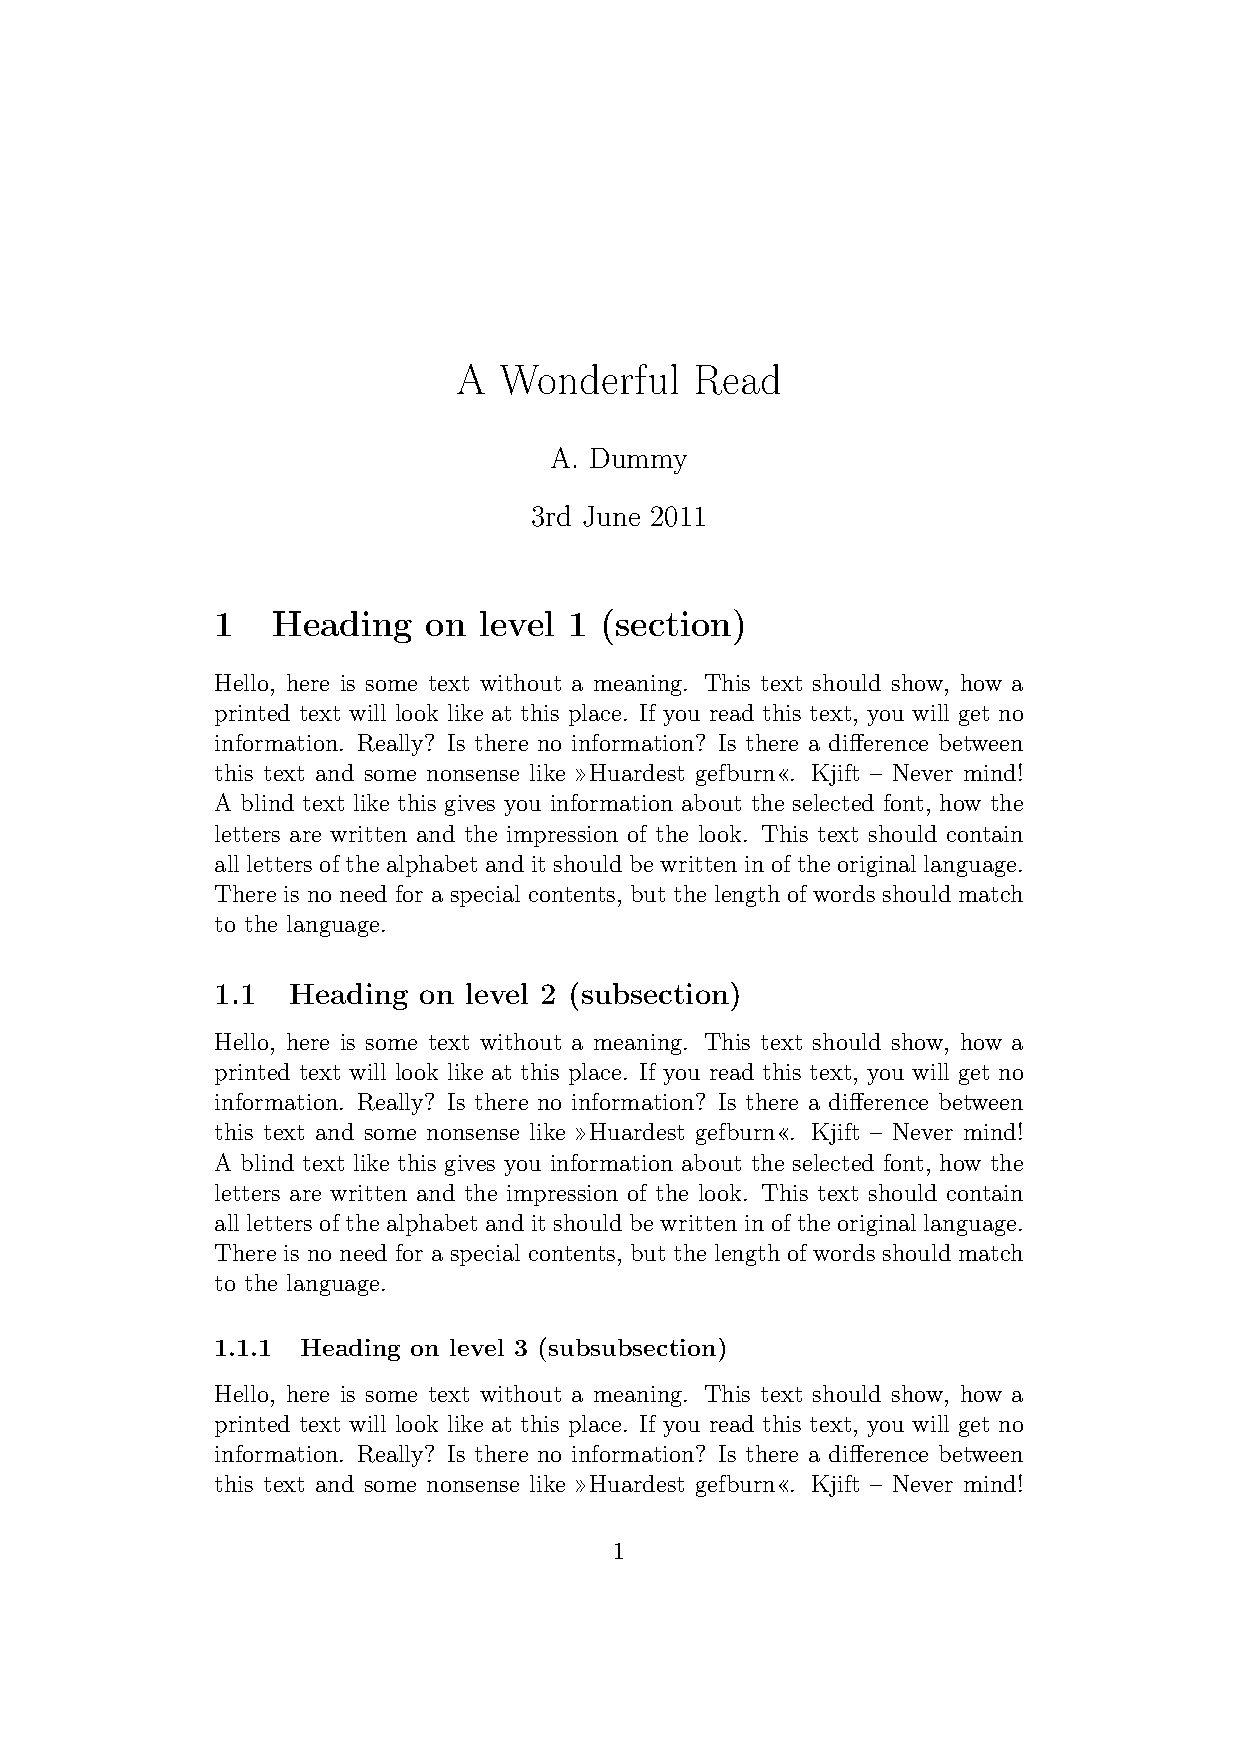
\includegraphics[width=.4\linewidth,page=1]{examples/basicarticle}}
\fcolorbox{black}{white}{\includegraphics[width=.4\linewidth,page=2]{examples/basicarticle}}
\fcolorbox{black}{white}{\includegraphics[width=.4\linewidth,page=3]{examples/basicarticle}}
\fcolorbox{black}{white}{\includegraphics[width=.4\linewidth,page=4]{examples/basicarticle}}
\end{column}
\end{columns}
\end{frame}

\begin{frame}[fragile]
\frametitle{Journal and Conference Proceedings Articles}
\begin{columns}[T]
\begin{column}{.33\textwidth}
\textsmaller{IEEE}\\\lstinline[basicstyle=\ttfamily\small]|\documentclass{IEEEtran}|
\vskip.5em
\fcolorbox{black}{white}{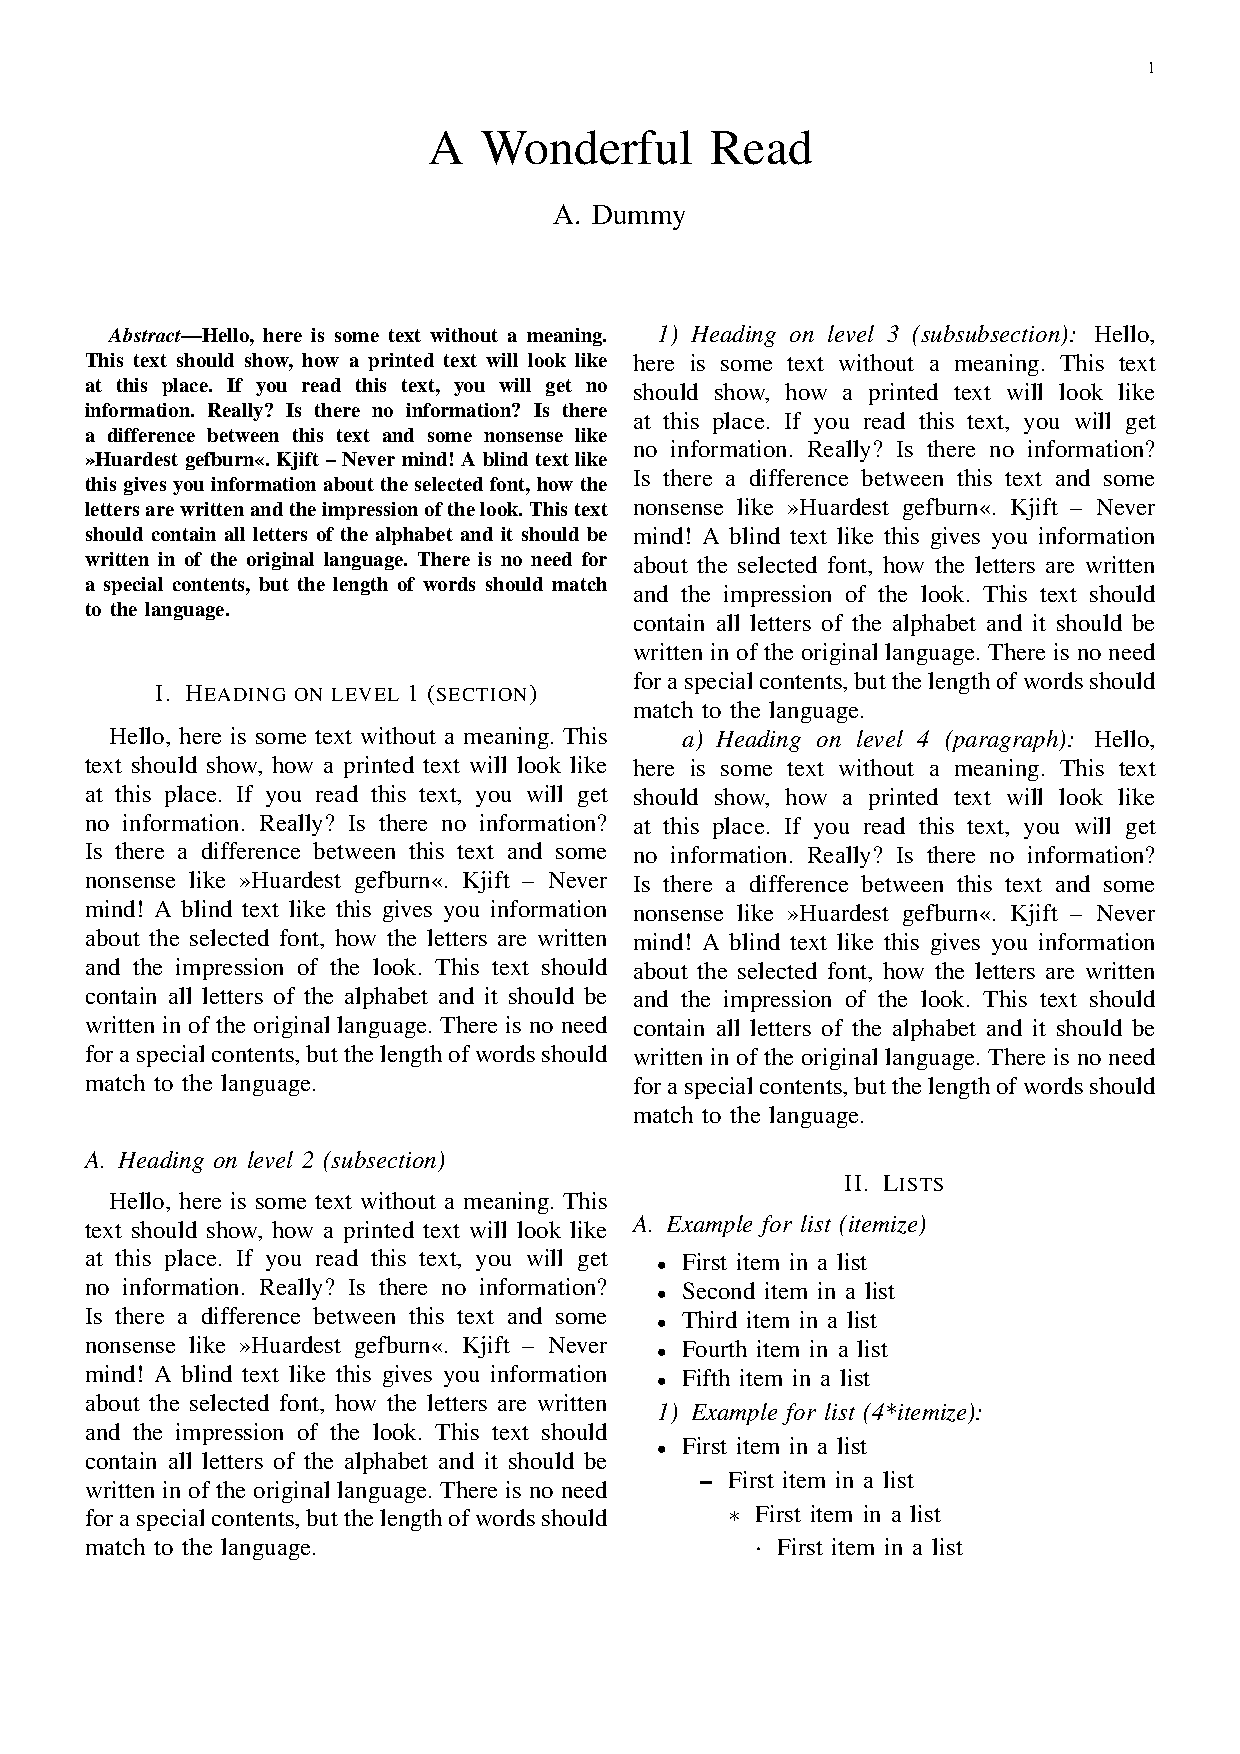
\includegraphics[width=\linewidth,page=1]{examples/IEEEtran}}
\end{column}

\begin{column}{.33\textwidth}
\textsmaller{ACM}\\\lstinline[basicstyle=\ttfamily\footnotesize\lsstyle,emphstyle=\scriptsize]|\documentclass{sig-alternate}|
\vskip.5em
\fcolorbox{black}{white}{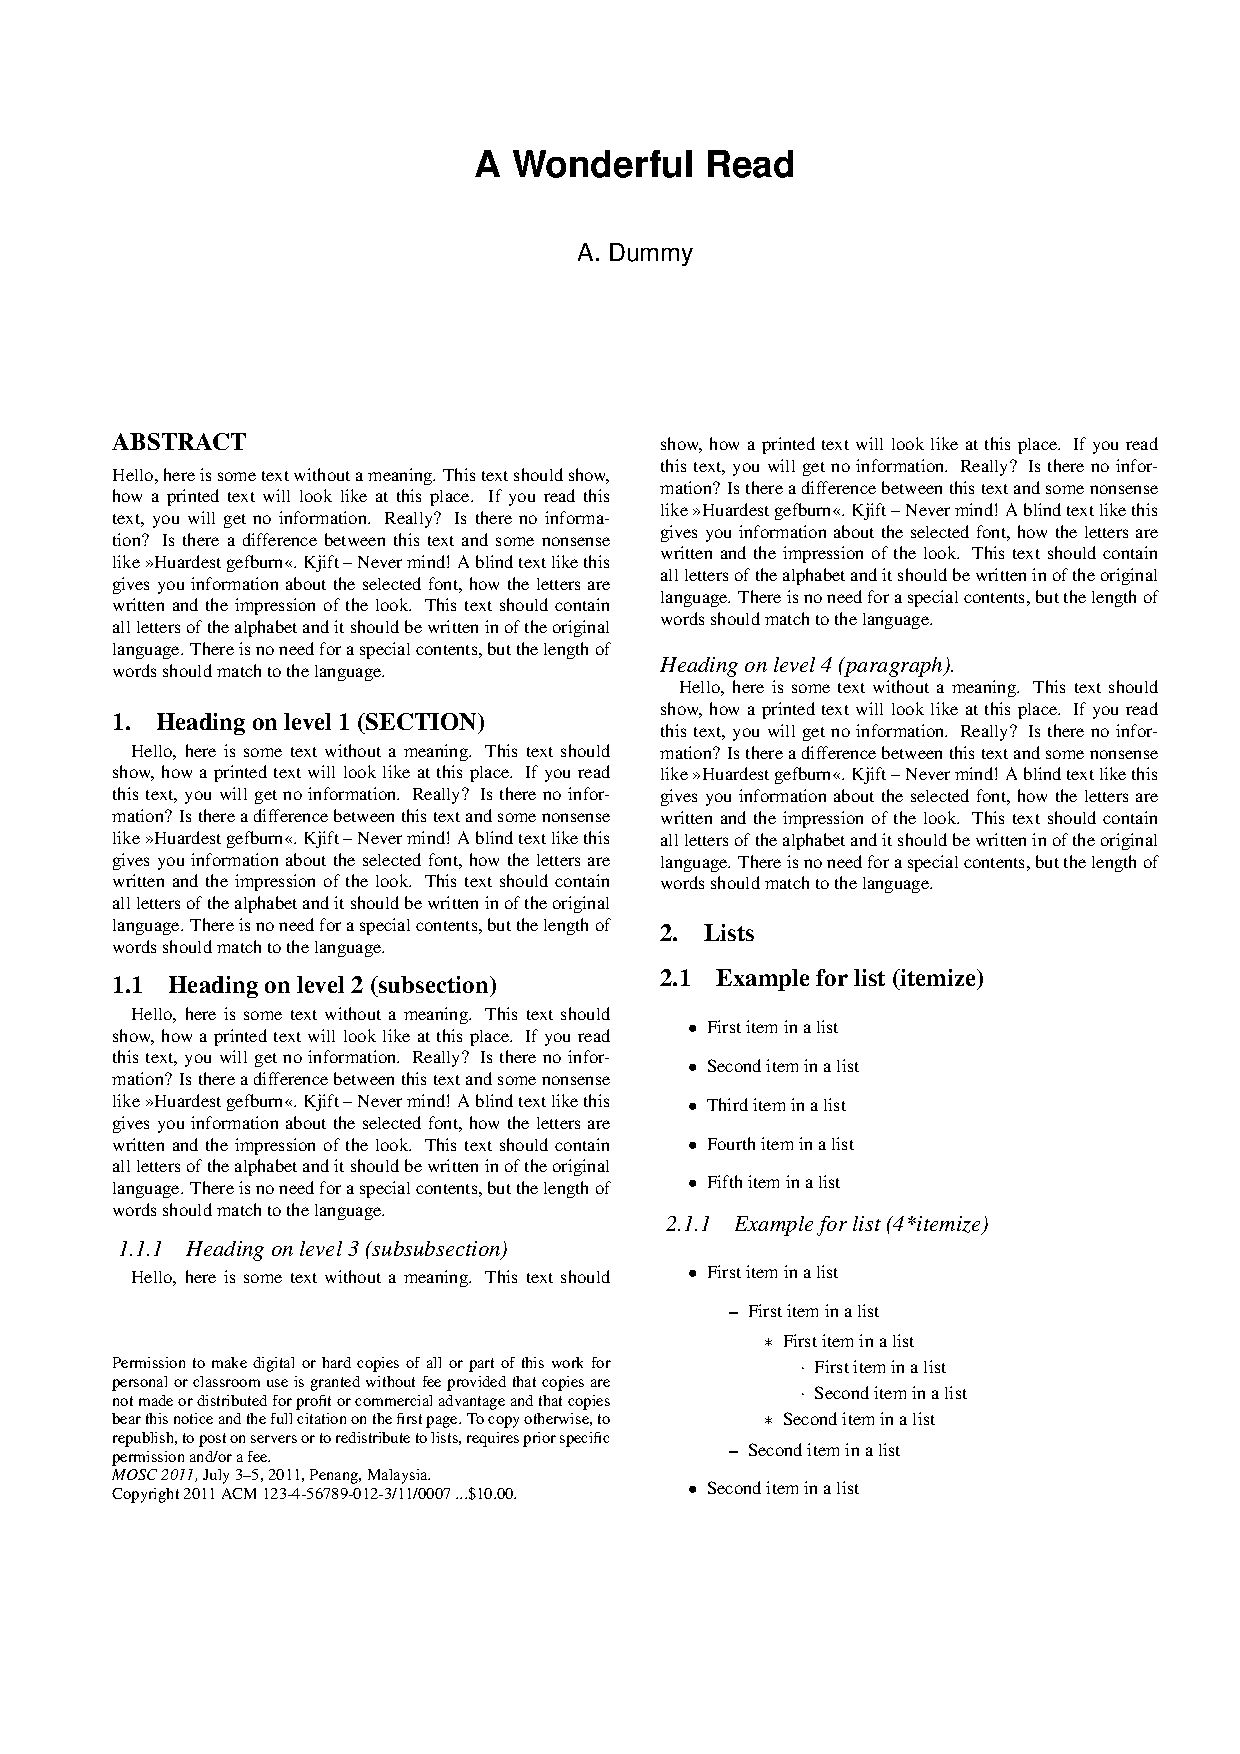
\includegraphics[width=\linewidth,page=1]{examples/acmconf}}
\end{column}

\begin{column}{.33\textwidth}
\textsmaller{LLNCS}\\\lstinline[basicstyle=\ttfamily\small]|\documentclass{llncs}|
\vskip.5em
\fcolorbox{black}{white}{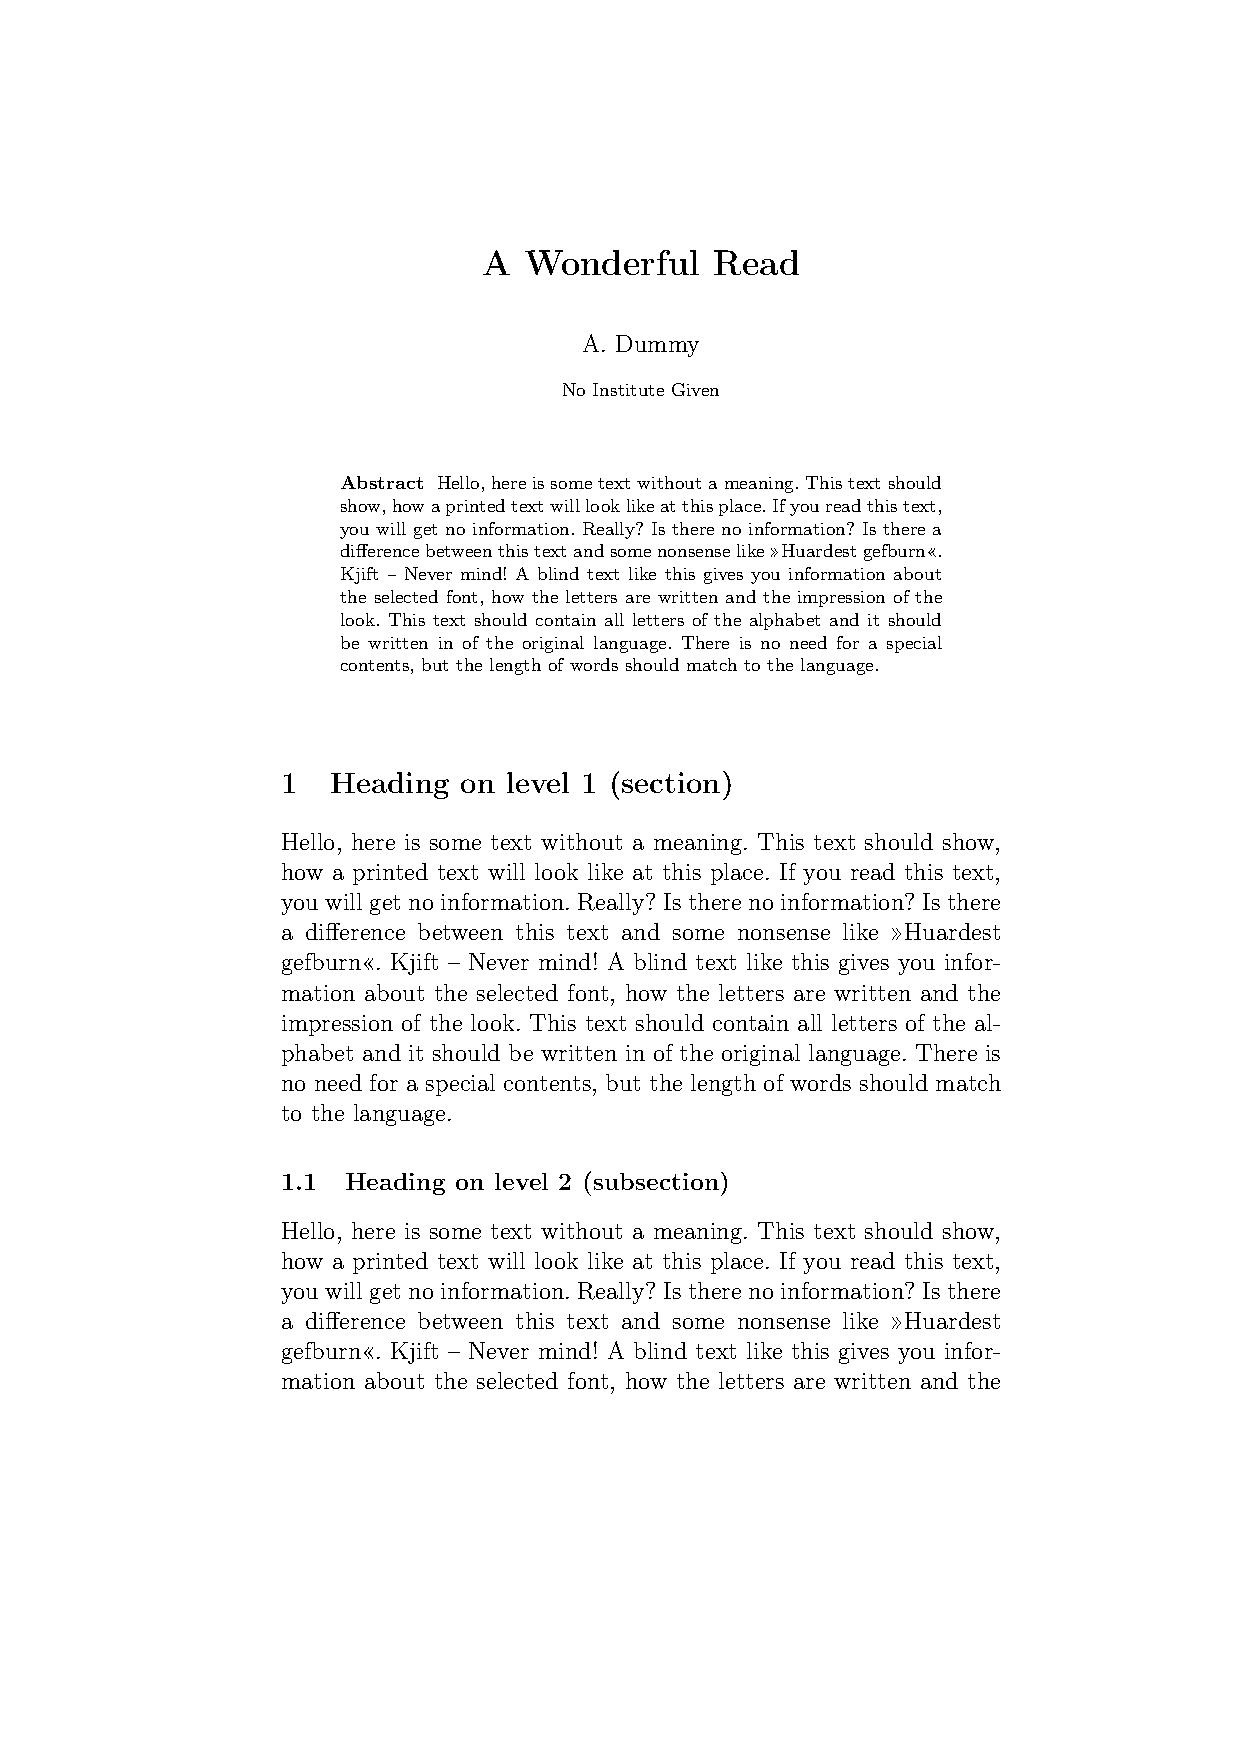
\includegraphics[width=\linewidth,page=1]{examples/llncs}}
\end{column}
\end{columns}
\end{frame}


\begin{frame}[fragile]
\lstset{basicstyle=\ttfamily}
\frametitle{Some Goodies}
\begin{itemize}
\item<+> Quick \structure{language-switching} with \texttt{babel}
\item<+> Automatic generation of \structure{cross-referencing labels}:\\
\lstinline|\section{Introduction}\label{sec:intro}|\\
\lstinline|... We saw in section \ref{sec:intro}...|
\item<+> Automatic generation of \structure{lists}:\\
\lstinline[texcs={tableofcontents}]|\tableofcontents|, \lstinline[texcs={listoffigures}]|\listoffigures|,  \lstinline[texcs={listoftables}]|\listoftables|
\item<+> Automatic generation of \structure{bibliographies} and \structure{indices}:\\
\lstinline|\cite{Knuth:1976}...\bibliography{references.bib}|\\
\lstinline[moretexcs={printindex}]|...the Linux kernel\index{Linux!kernel}... \printindex|\\
\item<+> Fully \structure{hyperlinked} \textsmaller{PDF} with bookmarks: \lstinline|\usepackage{hyperref}|
\item<+> Inclusion of selected pages from other \textsmaller{PDF}s\\(while inserting new page headers/footers!)\\
\lstset{basicstyle=\ttfamily\footnotesize,moretexcs={includepdf}}
\lstinline|\usepackage{pdfpages}|\\
\lstinline|\includepdf[pages={1,3-5,8},pagecommand=\thispagestyle{plain}]{file.pdf}|
\end{itemize}
\end{frame}


\begin{frame}[fragile,allowframebreaks]
\frametitle{University Theses}
\small
Universiti Sains Malaysia \lstinline[basicstyle=\ttfamily]|\documentclass{usmthesis}|
\vskip.5em

%% See http://liantze.penguinattack.org/latextypesetting.html#usmthesis
{\centering
\fcolorbox{black}{white}{\includegraphics[width=.24\linewidth,page=2]{examples/usmthesis.pdf}}
\fcolorbox{black}{white}{\includegraphics[width=.24\linewidth,page=4]{examples/usmthesis.pdf}}
\fcolorbox{black}{white}{\includegraphics[width=.24\linewidth,page=13]{examples/usmthesis.pdf}}
\fcolorbox{black}{white}{\includegraphics[width=.24\linewidth,page=36]{examples/usmthesis.pdf}}\par}

\pagebreak

%% See http://liantze.penguinattack.org/latextypesetting.html#mmuthesis
Multimedia University \lstinline[basicstyle=\ttfamily]|\documentclass{mmuthesis}|
\vskip.5em

{\centering
\fcolorbox{black}{white}{\includegraphics[width=.24\linewidth,page=3]{examples/mmuthesis.pdf}}
\fcolorbox{black}{white}{\includegraphics[width=.24\linewidth,page=9]{examples/mmuthesis.pdf}}
\fcolorbox{black}{white}{\includegraphics[width=.24\linewidth,page=13]{examples/mmuthesis.pdf}}
\fcolorbox{black}{white}{\includegraphics[width=.24\linewidth,page=18]{examples/mmuthesis.pdf}}
\par}

\pagebreak

%% See http://liantze.penguinattack.org/latextypesetting.html#umalayathesis
Universiti Malaya \lstinline[basicstyle=\ttfamily]|\documentclass{umalayathesis}|
\vskip.5em

{\centering
\fcolorbox{black}{white}{\includegraphics[width=.24\linewidth,page=2]{examples/umalayathesis.pdf}}
\fcolorbox{black}{white}{\includegraphics[width=.24\linewidth,page=6]{examples/umalayathesis.pdf}}
\fcolorbox{black}{white}{\includegraphics[width=.24\linewidth,page=12]{examples/umalayathesis.pdf}}
\fcolorbox{black}{white}{\includegraphics[width=.24\linewidth,page=20]{examples/umalayathesis.pdf}}
\par}

\end{frame}


\begin{frame}
\frametitle{Highly Configurable Documents}
\framesubtitle{\texttt{memoir} and \textsmaller{KOMA}-Script Classes}

\begin{itemize}
\item Sectional headings
\item Running headers and footers
\item Good font, colour and illustration choices
\item \url{http://latex-my.blogspot.com/search/label/bookdesign}
\end{itemize}

%% See http://liantze.penguinattack.org/ebooks.html
\begin{center}
\onslide<2>{%
%\fcolorbox{black}{white}{\includegraphics[width=.24\linewidth,page=1]{examples/GridComputingCluster-Report2009}}
%\fcolorbox{black}{white}{\includegraphics[width=.24\linewidth,page=5]{examples/GridComputingCluster-Report2009}}
%\fcolorbox{black}{white}{\includegraphics[width=.24\linewidth,page=10]{examples/GridComputingCluster-Report2009}}
%\fcolorbox{black}{white}{\includegraphics[width=.24\linewidth,page=32]{examples/GridComputingCluster-Report2009}}
%}
\fcolorbox{black}{white}{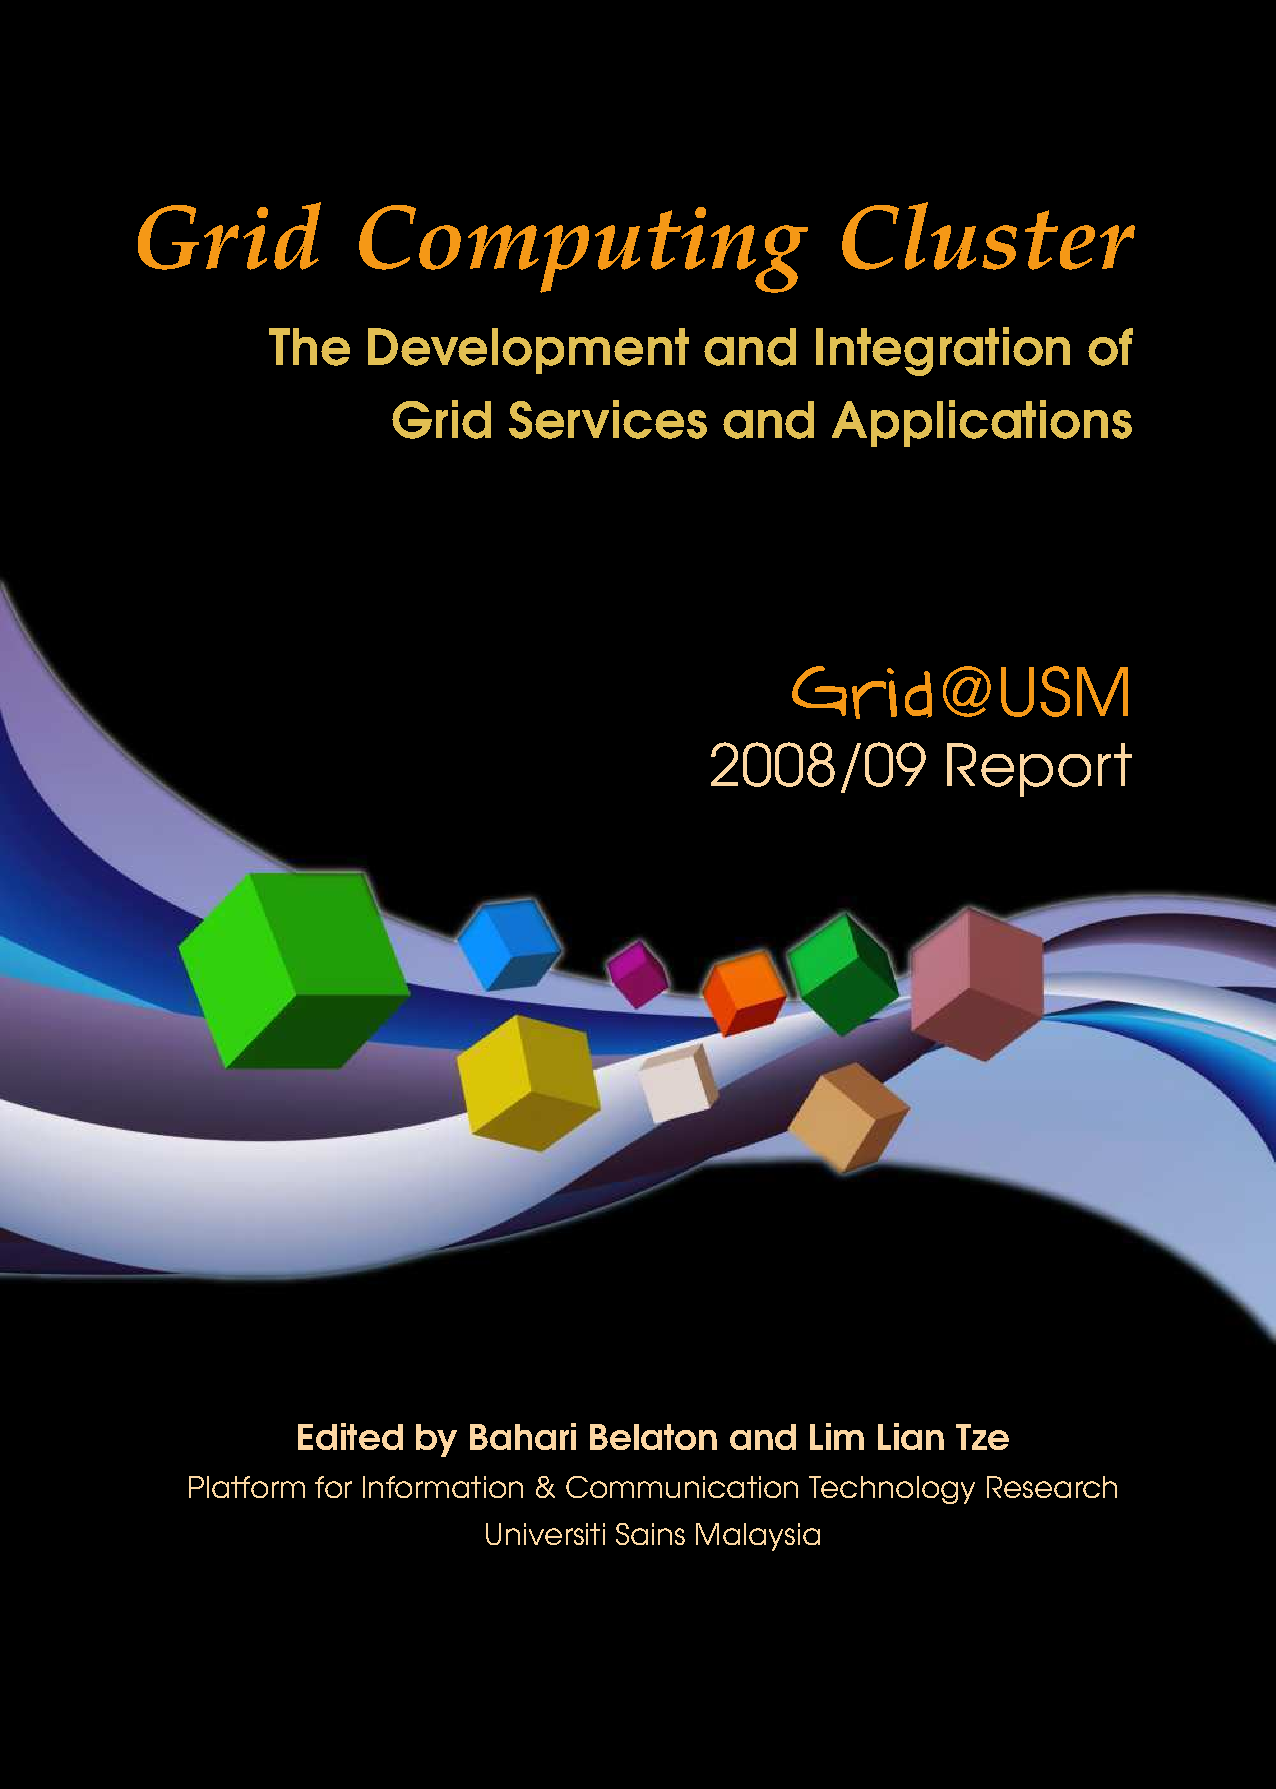
\includegraphics[width=.24\linewidth,page=1]{examples/GridBookExcerpt}}
\fcolorbox{black}{white}{\includegraphics[width=.24\linewidth,page=2]{examples/GridBookExcerpt}}
\fcolorbox{black}{white}{\includegraphics[width=.24\linewidth,page=3]{examples/GridBookExcerpt}}
\fcolorbox{black}{white}{\includegraphics[width=.24\linewidth,page=4]{examples/GridBookExcerpt}}
}
\end{center}
\end{frame}



\begin{frame}[fragile]
\frametitle{Presentation Slides}
\begin{itemize}
\item This presentation was made with \LaTeX!
\item<+-> Many possible classes: \texttt{powerdot}, \alert<2->{\texttt{beamer}}
\end{itemize}

\begin{columns}<+->
\begin{column}{.47\textwidth}
\begin{beamerboxesrounded}[width=\linewidth]{}
\vskip-1em
\begin{lstlisting}[basicstyle=\ttfamily\small,
moretexcs={usetheme,frametitle,frame,titleframe},
emph={beamer,frame},
escapechar={:},lineskip=-2pt]
\documentclass{beamer}
\usetheme{:\onslide<2>{Warsaw}%
\onslide<3|trans:0|handout:0>{\llap{Szeged}}%
\onslide<4|trans:0|handout:0>{\llap{Bergen}}%
\onslide<5|trans:0|handout:0>{\llap{oxygen}}:}

\author ...

\begin{document}
\titleframe

\section{Intro}

\begin{frame}
\frametitle{Some Background}
...
:\bfseries\color{Maroon}\textbackslash end:{frame}
\end{document}
\end{lstlisting}
\vspace*{-1em}
\end{beamerboxesrounded}
\end{column}
\begin{column}{.48\textwidth}
\centering
\onslide<2>{\fcolorbox{black}{white}{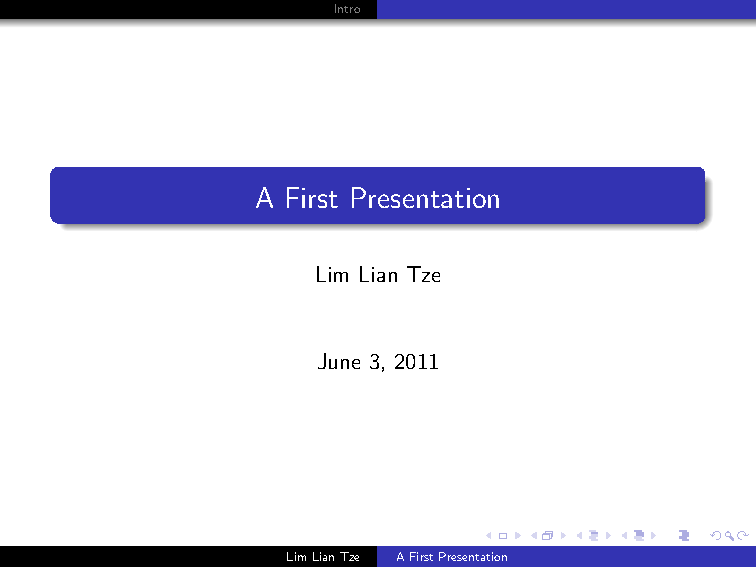
\includegraphics[width=.7\linewidth,page=1]{examples/beamer-Warsaw}}}%
\onslide<3|trans:0|handout:0>{\llap{\fcolorbox{black}{white}{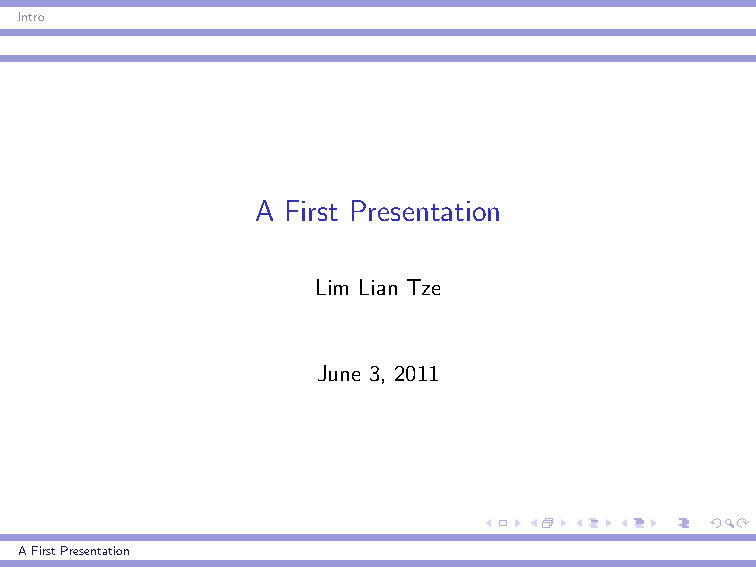
\includegraphics[width=.7\linewidth,page=1]{examples/beamer-Szeged}}
}}%
\onslide<4|trans:0|handout:0>{\llap{\fcolorbox{black}{white}{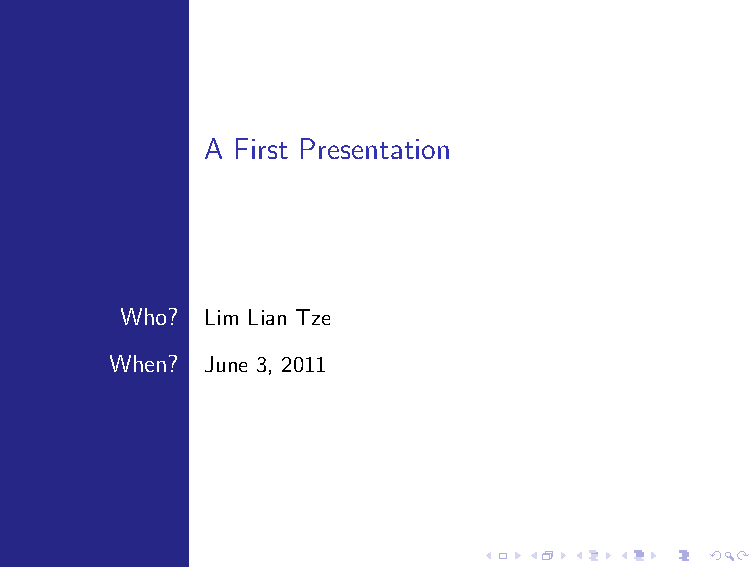
\includegraphics[width=.7\linewidth,page=1]{examples/beamer-Bergen}}
}}%
\onslide<5|trans:0|handout:0>{\llap{\fcolorbox{black}{white}{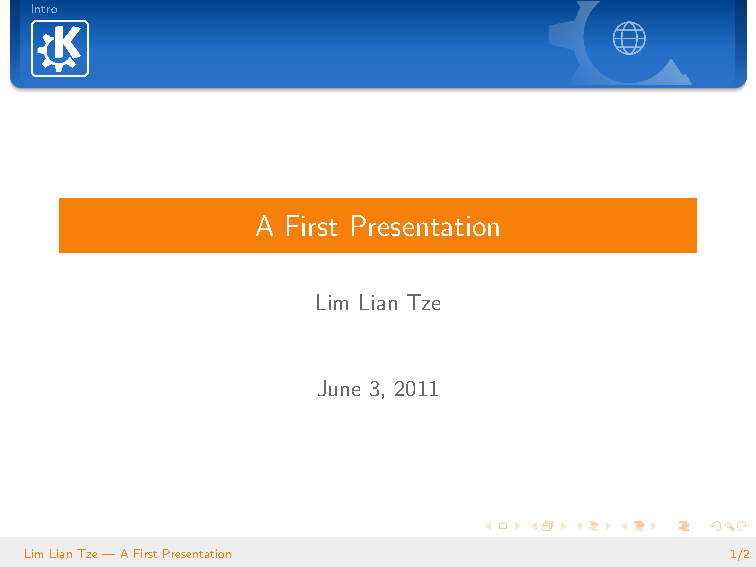
\includegraphics[width=.7\linewidth,page=1]{examples/beamer-Oxygen}}
}}

\onslide<2>{\fcolorbox{black}{white}{\includegraphics[width=.7\linewidth,page=2]{examples/beamer-Warsaw}}}%
\onslide<3|trans:0|handout:0>{\llap{\fcolorbox{black}{white}{\includegraphics[width=.7\linewidth,page=2]{examples/beamer-Szeged}}
}}%
\onslide<4|trans:0|handout:0>{\llap{\fcolorbox{black}{white}{\includegraphics[width=.7\linewidth,page=2]{examples/beamer-Bergen}}
}}%
\onslide<5|trans:0|handout:0>{\llap{\fcolorbox{black}{white}{\includegraphics[width=.7\linewidth,page=2]{examples/beamer-Oxygen}}
}}
\end{column}
\end{columns}
\end{frame}

\begin{frame}[fragile]
\frametitle{Oversized Posters}
\begin{itemize}
\item Many possible solutions: \texttt{sciposter}, \texttt{flowfram}, \alert<2->{\texttt{beamerposter}}
\end{itemize}

\begin{columns}<2->
\begin{column}{.5\textwidth}
\begin{beamerboxesrounded}[width=\linewidth]{}
\begin{lstlisting}[basicstyle=\ttfamily\small,
moretexcs={usetheme,frametitle,frame},
emph={beamer,beamerposter,frame},
escapechar={:},lineskip=-2pt]
\documentclass{beamer}
\usepackage[orientation=portrait, size=a0]{beamerposter}
\usetheme{...}
\author ... % Meta-information

\begin{document}
\begin{frame}
... % Poster contents goes here
:\bfseries\color{Maroon}\textbackslash end:{frame}
\end{document}
\end{lstlisting}
\end{beamerboxesrounded}
\end{column}
\begin{column}{.48\textwidth}
\centering
% See http://latex-my.blogspot.com/2011/03/creating-academic-posters-and-printing.html
\onslide<2>{\fcolorbox{black}{white}{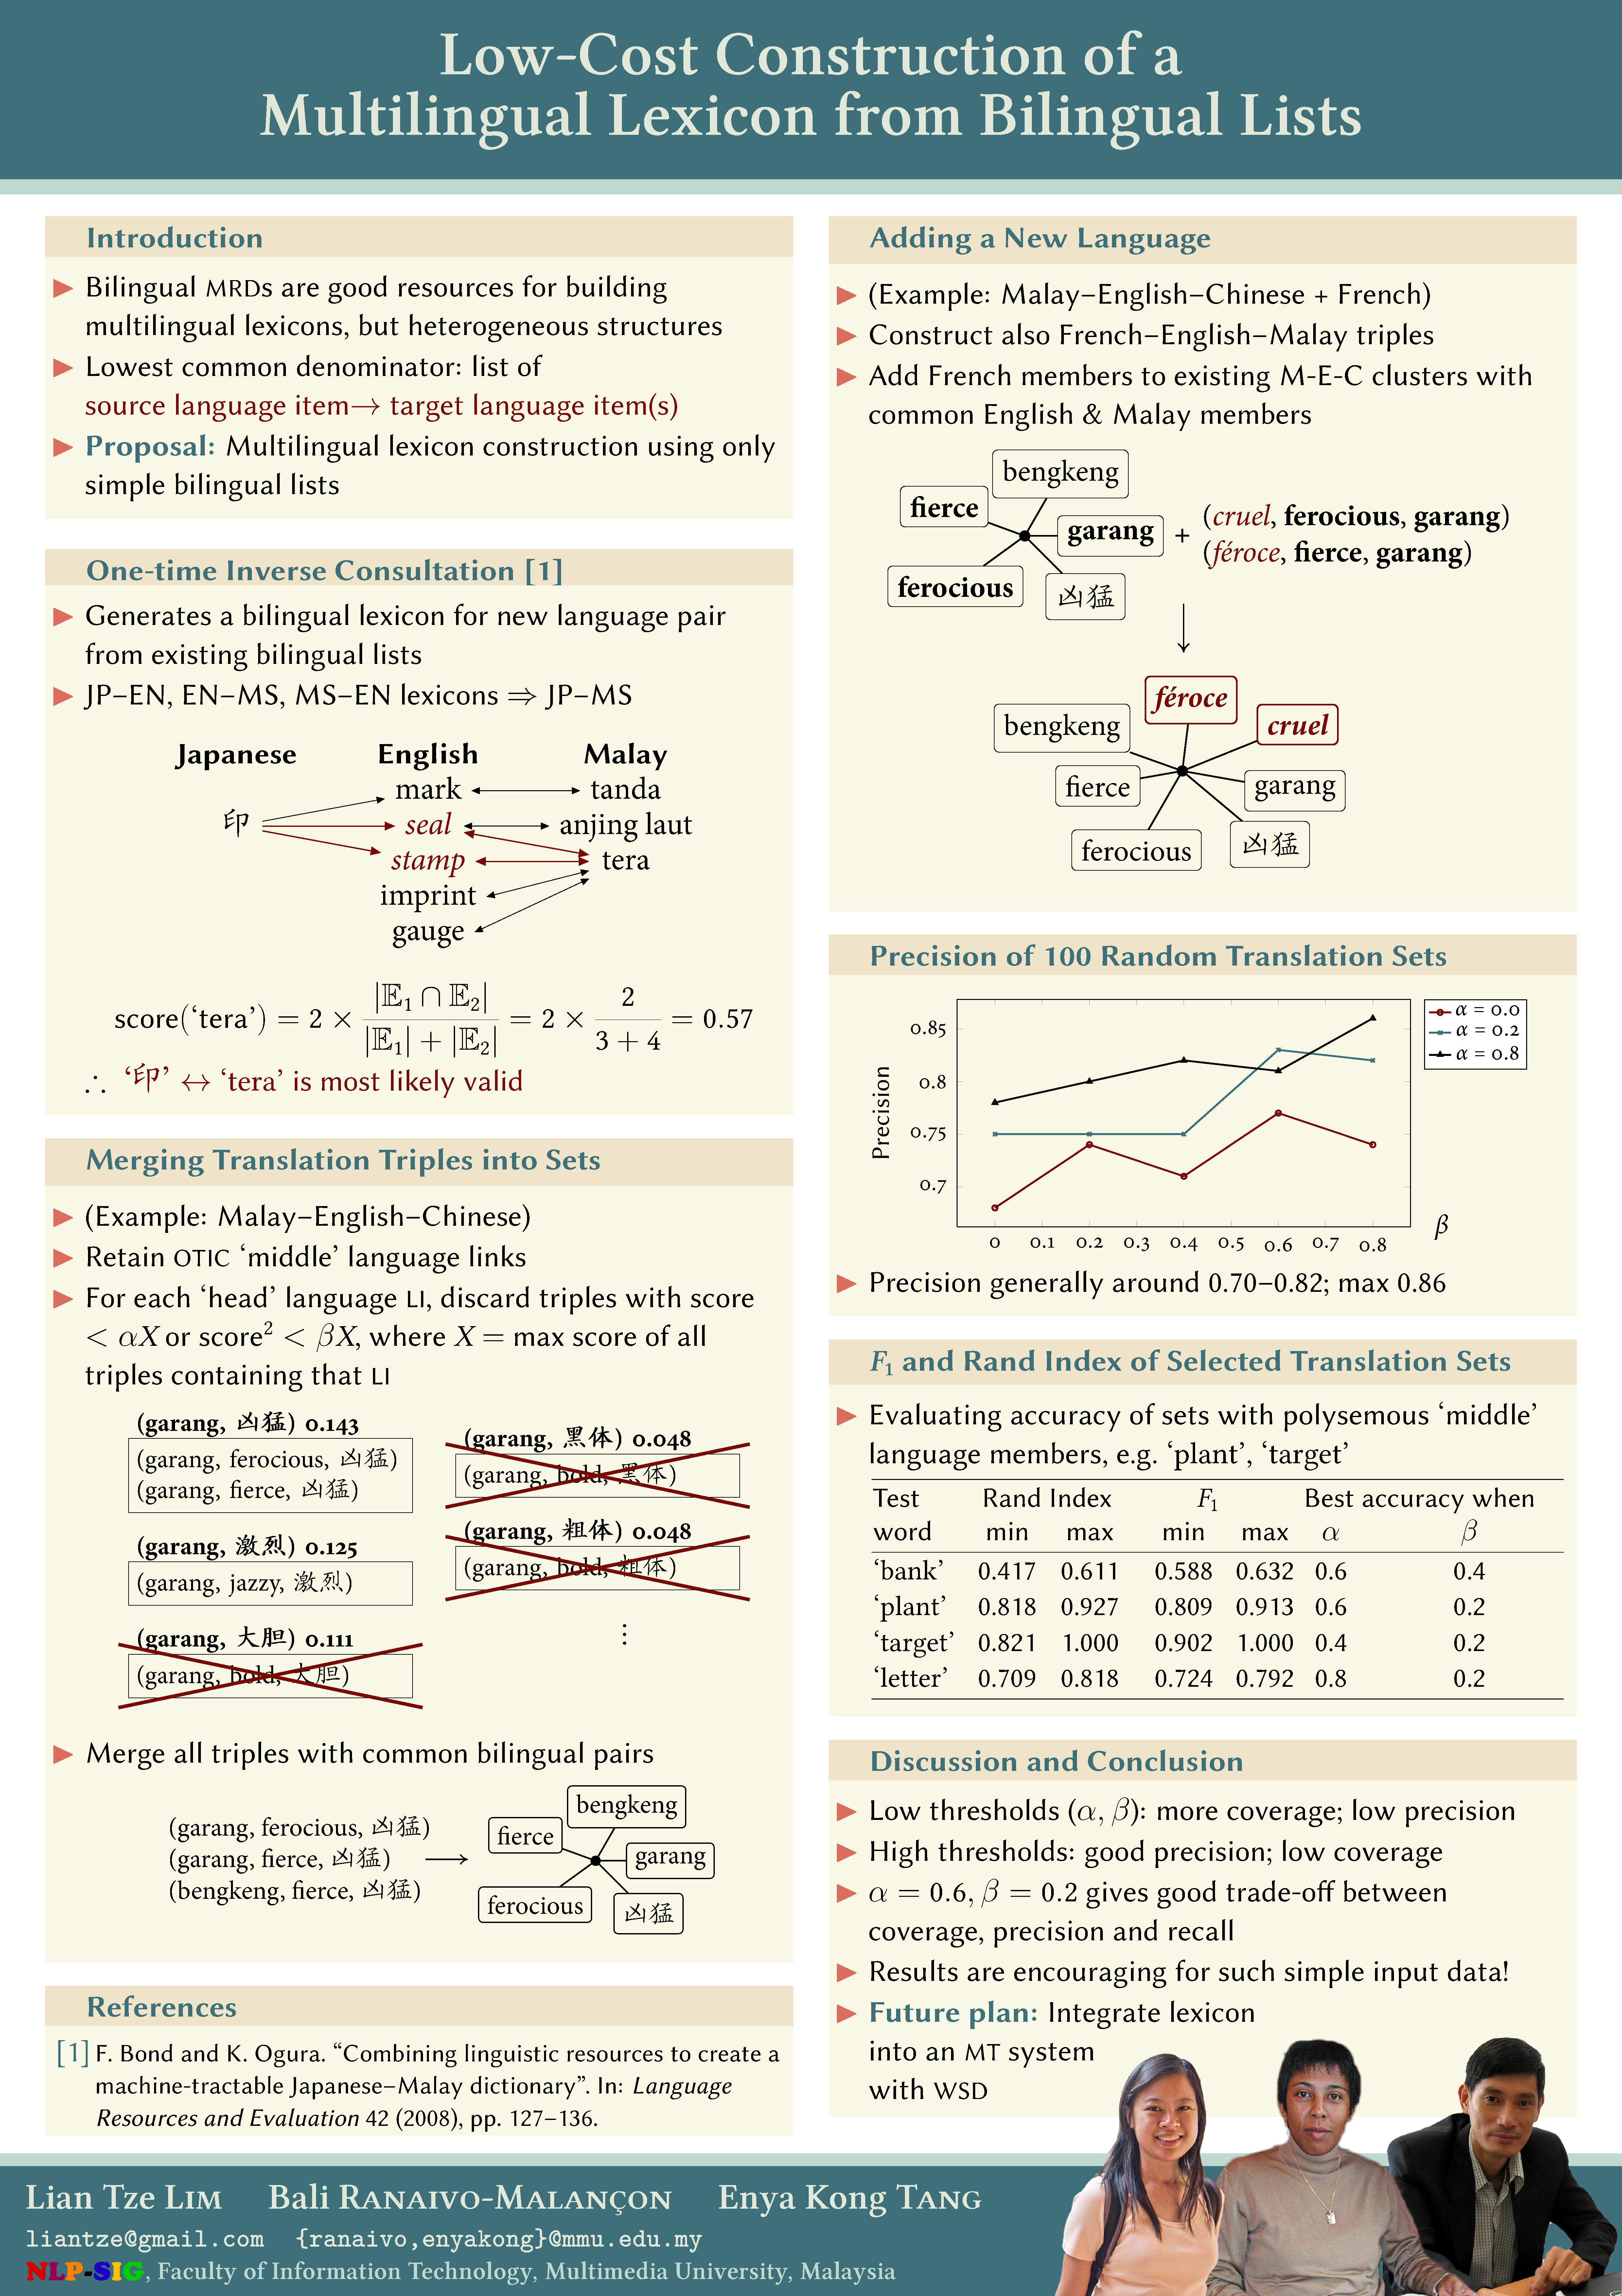
\includegraphics[width=.8\linewidth]{examples/cicling-poster-small.pdf}}}%
\onslide<3|trans:0|handout:0>{\llap{\fcolorbox{black}{white}{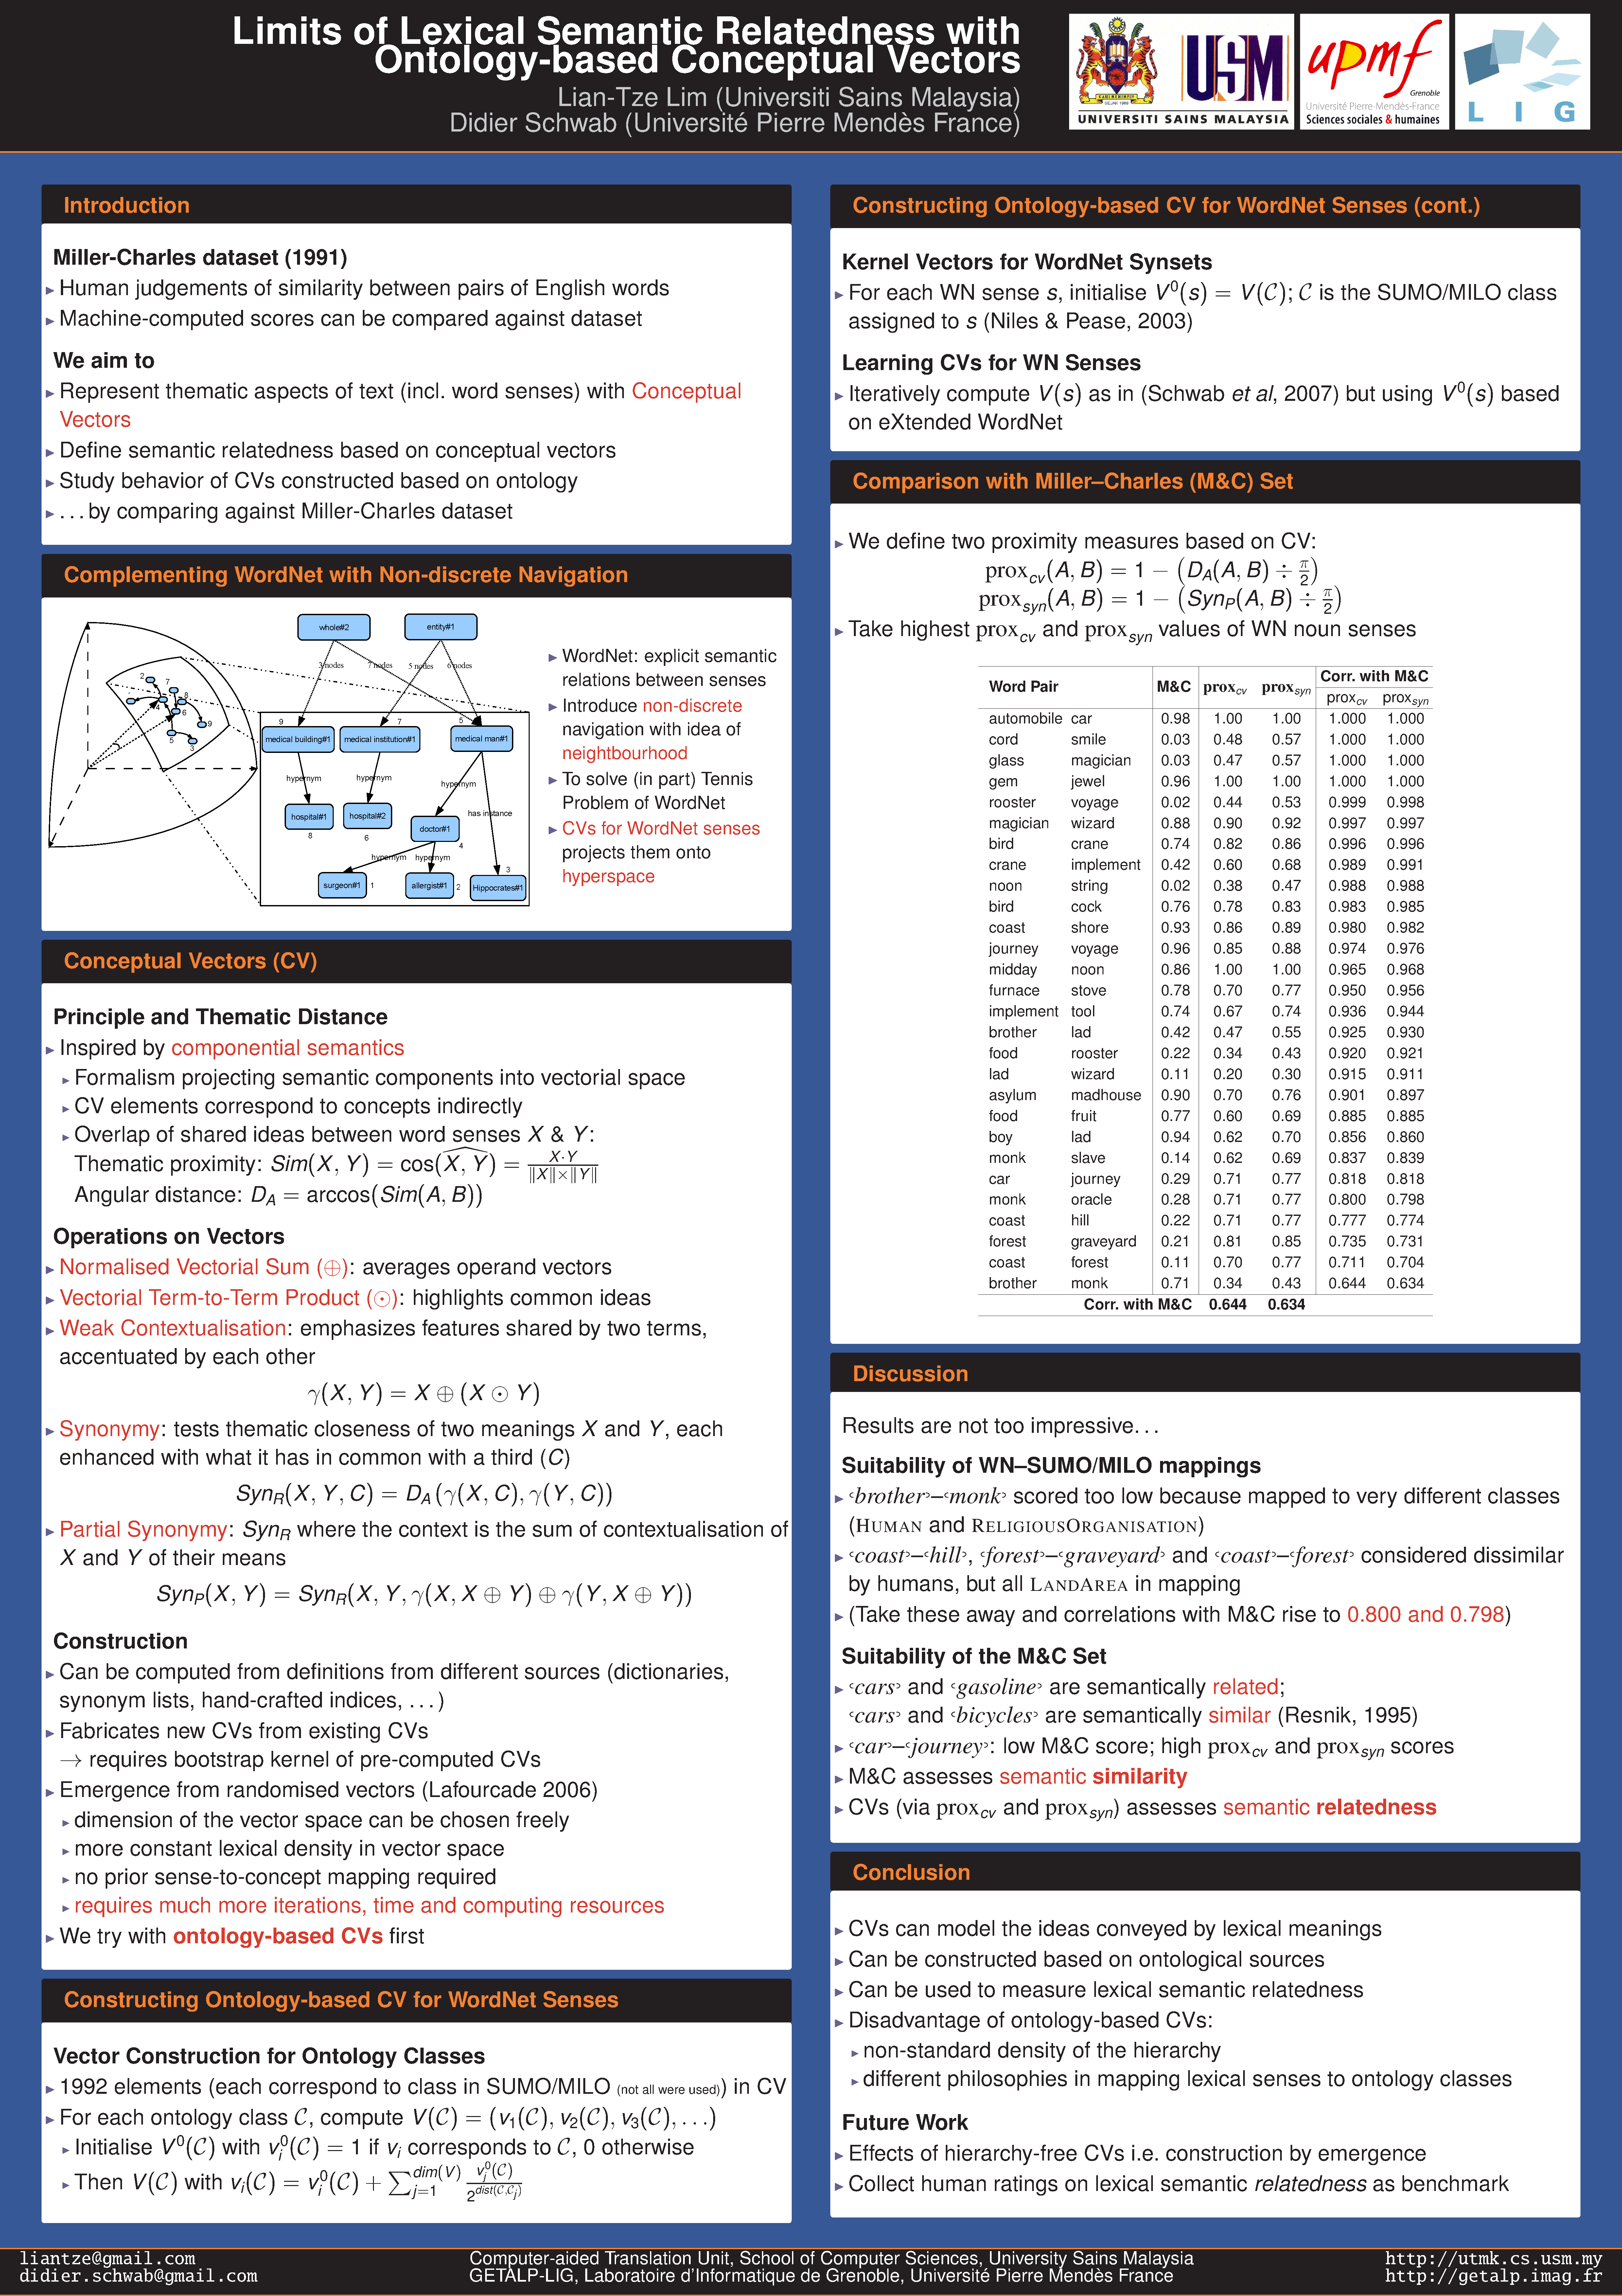
\includegraphics[width=.8\linewidth]{examples/NLPCS08-poster-small}}
}}
\end{column}
\end{columns}
\end{frame}


\begin{frame}[fragile]
\frametitle{Leaflets}

\begin{itemize}
\item \texttt{leaflet}: arrange contents into 6 pages on a foldable double-sided sheet
\end{itemize}

\begin{columns}
\begin{column}{.496\textwidth}
\begin{beamerboxesrounded}[width=\linewidth]{}
\begin{lstlisting}[basicstyle=\ttfamily\small,lineskip=-2pt,emph={leaflet},moretexcs={maketitle}]
\documentclass[foldmark,a4paper]
{leaflet}
\author ... % Meta-information

\begin{document}
\maketitle
\section ...
... % Leaflet contents
\end{document}
\end{lstlisting}
\end{beamerboxesrounded}
\end{column}
\begin{column}{.48\textwidth}
\centering
% See http://latex-my.blogspot.com/2011/04/making-leaflets-with-l-t-e-x.html
\fcolorbox{black}{white}{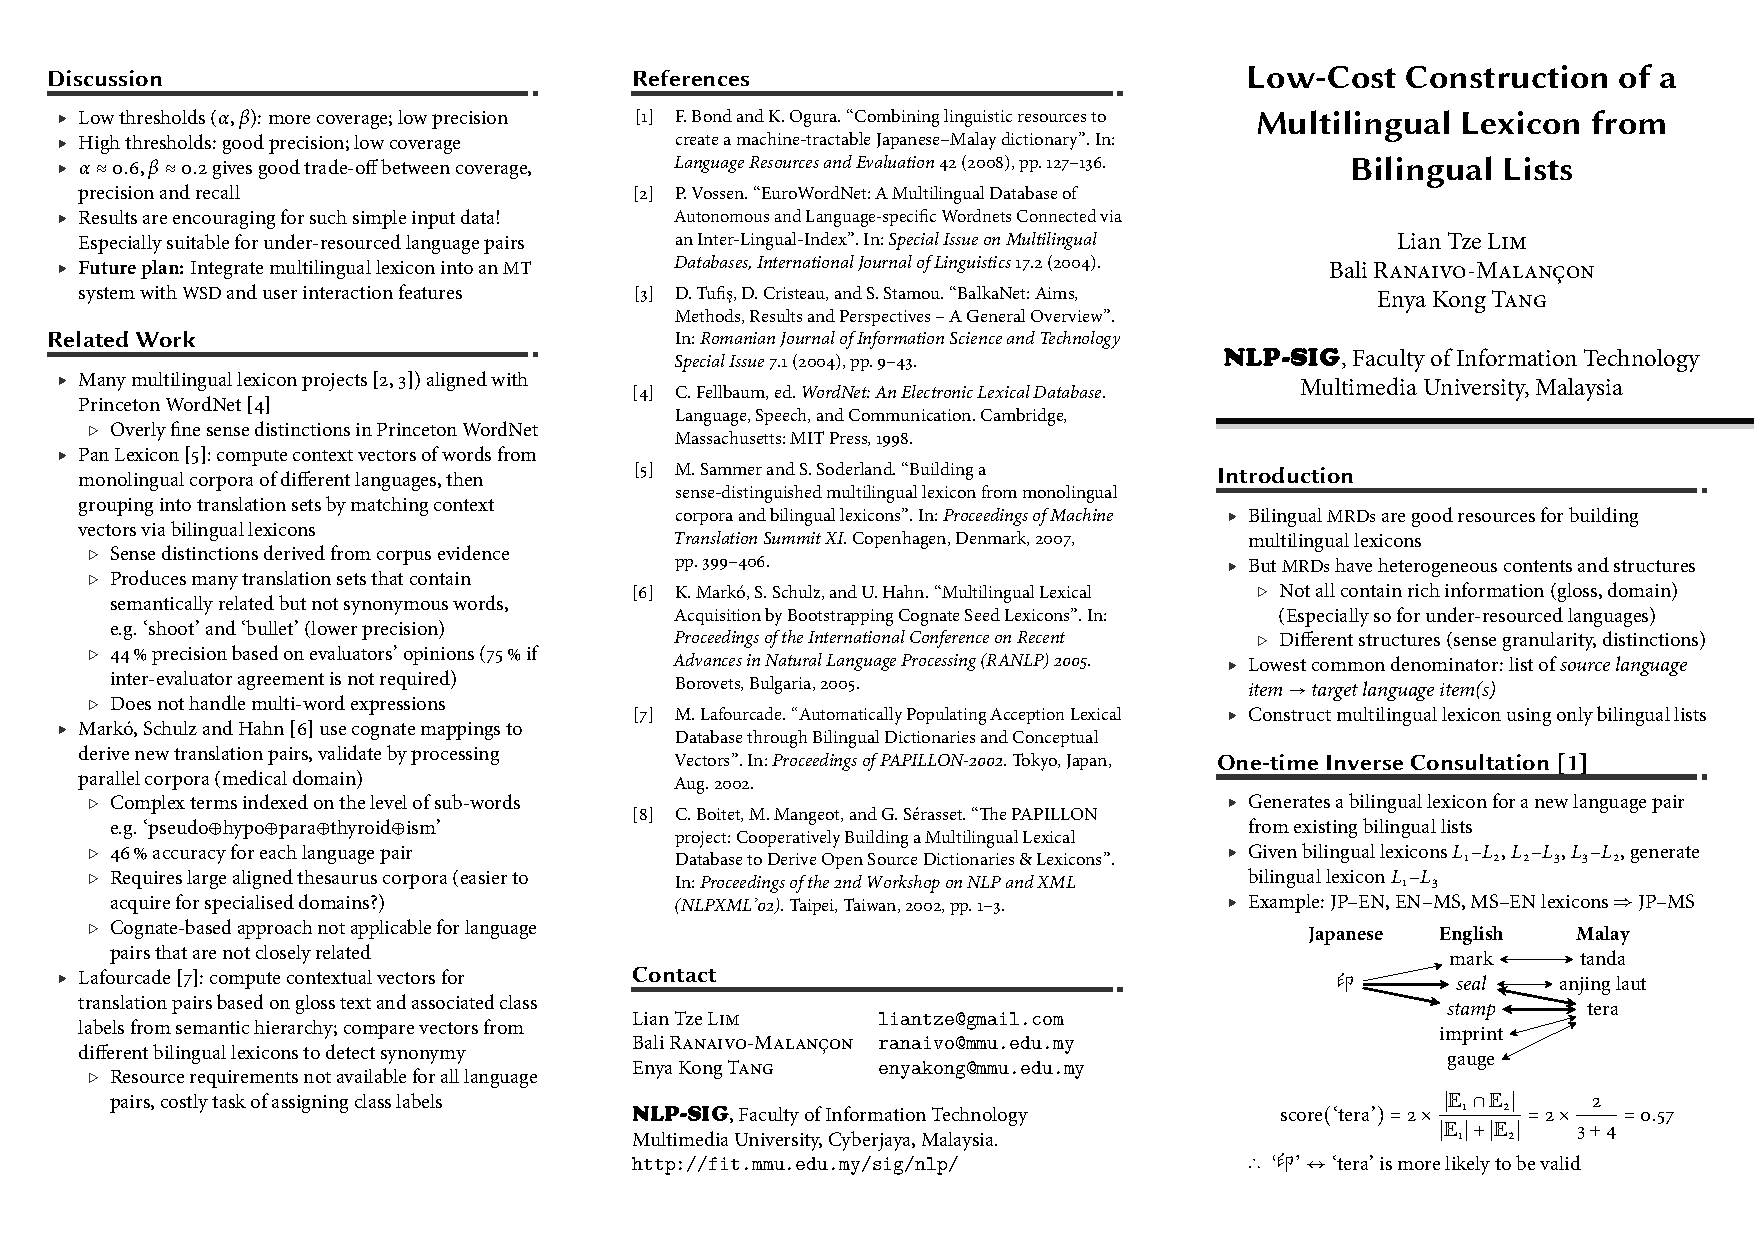
\includegraphics[width=.85\linewidth,page=1]{examples/cicling-handout.pdf}}
\fcolorbox{black}{white}{\includegraphics[width=.85\linewidth,page=2]{examples/cicling-handout.pdf}}\par
\end{column}
\end{columns}

\end{frame}


\begin{frame}[fragile,allowframebreaks]
\frametitle{Fillable \textsmaller{PDF} Forms}
\begin{columns}
\begin{column}{.52\textwidth}
\begin{beamerboxesrounded}{}
\begin{lstlisting}[basicstyle=\ttfamily\small,escapechar=|,
moretexcs={TextField,ChoiceMenu,CheckBox},
emph={hyperref}]
\usepackage{hyperref}
... % various settings skipped
\TextField{Name:}\\
\TextField{Affiliation:}\\
\ChoiceMenu[radio=true]
{Are you a:}{Student, Academic}\\
Interest:
\CheckBox{Security}
\CheckBox{Systems}
\CheckBox{User space}\\
\TextField[multiline=true]
{Comments:}\\
\end{lstlisting}
\end{beamerboxesrounded}
\end{column}
\begin{column}{.47\textwidth}
\centering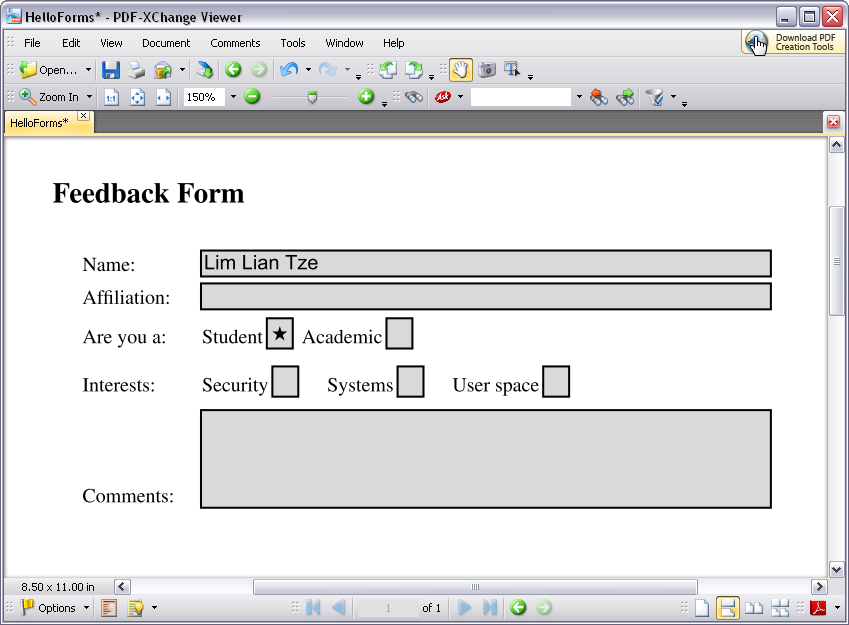
\includegraphics[width=\linewidth]{examples/form-screencap}\par
\end{column}
\end{columns}
\pagebreak

\alert{Use with caution!}
\begin{itemize}
\item \texttt{poppler}-based viewers (\texttt{evince}, \texttt{xpdf}, \texttt{okular})
\begin{itemize}
\item Problem displaying and saving radio/check boxes correctly
\item Saved forms can't be opened by other viewers
\end{itemize}
\item Adobe Reader
\begin{itemize}
\item Cannot save filled form as \textsmaller{PDF} unless Acrobat is installed
\item Only as field-and-value text file
\item Can provide ``Submit'' button for submission to a \textsmaller{URL}
\item Or print hard copy of filled form!
\end{itemize}
\item PDF XChange Viewer
\begin{itemize}
\item Best freeware for filling and saving \LaTeX-created forms
\item Windows only
\item Not \textsmaller{OSS}
\end{itemize}
\end{itemize}

\end{frame}


\begin{frame}[fragile]
\frametitle{Flash Cards}
\begin{columns}
\begin{column}{.465\textwidth}
\begin{beamerboxesrounded}{}
\vskip-1em
\begin{lstlisting}[basicstyle={\ttfamily\small},
emph={flashcards,flashcard},
moretexcs={cardfrontstyle,cardfrontfoot}]
\documentclass[avery5388,frame]
{flashcards}
\cardfrontstyle{headings}
\cardfrontfoot{Linux}

\begin{document}
\begin{flashcard}[Security]
{Certificate}
...
\end{flashcard}

\begin{flashcard}[Security]
{MAC ...}
...
\end{flashcard}
\end{document}
\end{lstlisting}
\vspace*{-1em}
\end{beamerboxesrounded}
\end{column}

\begin{column}{.53\textwidth}
\centering
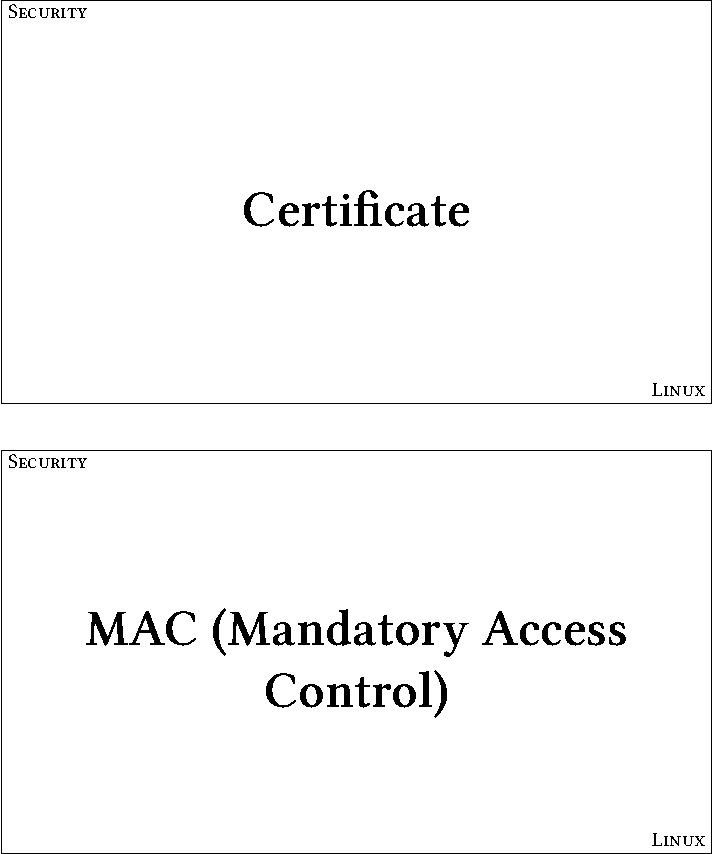
\includegraphics[width=.49\linewidth,page=1]{examples/flashcard-crop}\hfill
\includegraphics[width=.49\linewidth,page=2]{examples/flashcard-crop}
\par
\end{column}
\end{columns}
\end{frame}


\begin{frame}[fragile]
\frametitle{Examination Questions}
\begin{columns}[T]
\begin{column}{.49\textwidth}
\begin{beamerboxesrounded}{}
\vskip-1em
\begin{lstlisting}[moretexcs={question,choice,CorrectChoice,part,printanswers},
emph={exam,questions,oneparchoices,parts,solution},
basicstyle=\ttfamily\scriptsize\lsstyle,lineskip=-1pt,escapechar=;]
\documentclass{exam}
...
\begin{questions};\onslide<2>{\bfseries\color{Maroon}\textbackslash printanswers};
\question[5] 
What is Paul McCartney's middle name?
\begin{oneparchoices}
\choice John \CorrectChoice Paul 
\choice Ringo \choice James
\end{oneparchoices}

\question[10] What was the Beatles' first single in 1962?
\begin{solution}Love Me Do\end{solution}

\question
\begin{parts} 
\part[5] What was George's inspiration for `While My Guitar Gently Weeps'?
\begin{solution}
He opened a random book and saw the words ``gently weep''.
\end{solution} 
...
\end{questions}
\end{lstlisting}
\vspace{-1em}
\end{beamerboxesrounded}
\end{column}
\begin{column}{.49\textwidth}
\centering
\onslide<1|trans:0|handout:0>{\fcolorbox{black}{white}{\includegraphics[width=\linewidth,page=1]{examples/exam}}}%
\onslide<2>{\llap{\fcolorbox{black}{white}{\includegraphics[width=\linewidth,page=2]{examples/exam}}}}
\end{column}
\end{columns}
\end{frame}

% !TEX root=talk.tex
\section{Special Material}

\begin{frame}[fragile]
\frametitle{Mathematics}
\begin{center}\begin{minipage}{.7\textwidth}\rmfamily
\eqref{eq:gratio} relates the golden ratio and the Fibonacci series.  Recall that the golden ratio, $\phi = \frac{1}{2} (1 + \sqrt{5})$.

\begin{equation}\label{eq:gratio}
\phi = 1 + \sum^{\infty}_{n=1}
                \frac{ (-1)^{n+1} }{ F_n F_{n+1} }
\end{equation}
\end{minipage}
\end{center}

\begin{beamerboxesrounded}{}
\vskip-1em
\begin{lstlisting}[escapechar=|,basicstyle=\ttfamily\small,moretexcs=eqref,emph={equation}]
\eqref{eq:gratio} relates the golden ratio and the Fibonacci series. 
Recall that the golden ratio, |\textcolor{red}{\large\ttfamily\$}|\phi = \frac{1}{2} (1 + \sqrt{5})|\textcolor{red}{\large\ttfamily\$}|.

\begin{equation}\label{eq:gratio}
\phi = 1 + \sum^{\infty} _{n=1}
                \frac{ (-1)^{n+1} }{ F_n F_{n+1} }
\end{equation}
\end{lstlisting}
\vspace*{-1em}
\end{beamerboxesrounded}
\end{frame}

\begin{frame}[fragile]
\frametitle{Chemical Equations and Molecules}

\begin{center}\rmfamily\small
\ce{Zn^2+ <=>[\ce{+ 2OH-}][\ce{+ 2H+}]
$\underset{\text{amphoteres Hydroxid}}{\ce{Zn(OH)2 v}}$
<=>C[+2OH-][{+ 2H+}]
$\underset{\text{Hydroxozikat}}{\cf{[Zn(OH)4]^2-}}$
}
\hfil
\chemfig{H-C(-[2]H)(-[6]H)-C(-[7]H)=[1]O}
\end{center}

\begin{beamerboxesrounded}{}
\vskip-1em
\begin{lstlisting}[basicstyle=\ttfamily\small,moretexcs={ce,chemfig,underset,text,cf},
emph={mhchem,chemfig}]
\usepackage[version=3]{mhchem}   % sufficient for chemical equations
\usepackage{chemfig}   % for 2-D molecule drawings
...
\ce{Zn^2+ <=>[\ce{+ 2OH-}][\ce{+ 2H+}]
$\underset{\text{amphoteres Hydroxid}}{\ce{Zn(OH)2 v}}$
<=> C[+2OH-][{+ 2H+}] 
$\underset{\text{Hydroxozikat}}{\cf{[Zn(OH)4]^2-}}$ }

\chemfig{H-C(-[2]H)(-[6]H)-C(-[7]H)=[1]O}
\end{lstlisting}
\vspace*{-1em}
\end{beamerboxesrounded}

\end{frame}

\begin{frame}[fragile]
\frametitle{Linguistics}

\begin{columns}
\begin{column}{.54\textwidth}\small\rmfamily
\exg. \%*Wen liebt seine Mutter?\\
Whom loves his mother\\
`Who does his mother love?'

\exi. [[NP He ] [VP kicked [NP the ball ]]]S

\end{column}
\begin{column}{.45\textwidth}\footnotesize\rmfamily
\Tree [ .S [.NP [.Pron He ] ] [.VP [.V kicked ] [.NP [.Det the ] [.N ball ] ] ] ]
\end{column}
\end{columns}

\medskip

\begin{beamerboxesrounded}{}
\vskip-1em
\begin{lstlisting}[moretexcs={exg,exi,Tree},basicstyle=\ttfamily\small\lsstyle,
emph={linguex,qtree},
lineskip=-2pt,commentstyle={}]
\usepackage{linguex,qtree}
...
\exg. \%*Wen liebt seine Mutter?\\
Whom loves his mother\\
`Who does his mother love?'

\exi. [[NP He ] [VP kicked [NP the ball ]]]S

\Tree [ .S [.NP [.Pron He ] ] [.VP [.V kicked ] [.NP [.Det the ] [.N ball ] ] ] ]
\end{lstlisting}
\vspace*{-1em}
\end{beamerboxesrounded}

\end{frame}


\begin{frame}[fragile]
\frametitle{Program Listings}

\begin{columns}
\begin{column}{.5\textwidth}
\begin{beamerboxesrounded}{}
\vspace{-1em}
\begin{lstlisting}[basicstyle=\ttfamily\footnotesize,
emph={listings,lstlisting},moretexcs={color}]
\usepackage{listings,xcolor}
...
\begin{lstlisting}
[language=C,columns=fullflexible,
basicstyle=\ttfamily,
keywordstyle=\bfseries\color{red},
commentstyle=\sffamily\color{green},
stringstyle=\rmfamily\color{orange}]
#include <stdio.h>
/* 
 | Prints "hello world"
 */
int main(void)
{
    printf("hello, world\n");
    return 0;
}
:\bfseries\color{Maroon}\textbackslash end:{lstlisting}
\end{lstlisting}
\vspace{-1em}
\end{beamerboxesrounded}
\end{column}
\hfill\begin{column}{.46\textwidth}
\begin{lstlisting}[language=C,escapechar=~,lineskip=-2pt,
basicstyle=\ttfamily,
commentstyle=\upshape\sffamily\small\color{SeaGreen4},keepspaces=true,
keywordstyle=\bfseries\color{Maroon},stringstyle=\rmfamily\color{Sienna2}]
#include <stdio.h>

/* 
 | Prints "hello world"
 */
int main(void)
{
    printf("hello, world\n");
    return 0;
}
\end{lstlisting}
\end{column}
\end{columns}
\end{frame}

\begin{frame}[fragile]
\frametitle{Network Protocols}
\begin{columns}
\begin{column}{.505\textwidth}
\begin{beamerboxesrounded}{}
\vspace{-1em}
\begin{lstlisting}[basicstyle=\ttfamily\footnotesize,
moretexcs={bitheader,wordgroupr,bitbox,endwordgroupr,wordbox},
emph={bytefield}]
\usepackage{bytefield}
...
\begin{bytefield}{16} 
\bitheader{0,7,8,15} \\ 
\wordgroupr{Header} 
\bitbox{4}{Tag} & \bitbox{12}{Mask} \\ 
\bitbox{8}{Source} & 
\bitbox{8}{Destination} 
\endwordgroupr \\ 
\wordbox{3}{Data} 
\end{bytefield} 
\end{lstlisting}
\vspace{-1em}
\end{beamerboxesrounded}
\end{column}
\begin{column}{.49\textwidth}\rmfamily\small
\hfill\begin{bytefield}{16}
\bitheader{0,7,8,15} \\ 
\wordgroupr{Header} 
\bitbox{4}{Tag} & \bitbox{12}{Mask} \\ 
\bitbox{8}{Source} & \bitbox{8}{Destination} 
\endwordgroupr \\ 
\wordbox{3}{Data} 
\end{bytefield} 
\end{column}
\end{columns}
\end{frame}

\begin{frame}[fragile]
\frametitle{Life Sciences}

\begin{texshade}{examples/AQPpro.MSF}
\shadingmode{similar} 
\threshold[80]{50} 
\setends{1}{80..112} 
\hideconsensus 
\feature{top}{1}{93..93}{fill:$\downarrow$}{first case (see text)} 
\feature{bottom}{1}{98..98}{fill:$\uparrow$}{second case (see text)} 
\end{texshade}
\vskip-1em
\begin{beamerboxesrounded}{}
\vskip-1em
\begin{lstlisting}[
moretexcs={setends,shadingmode,threshold,hideconsensus,feature,downarrow,uparrow},
emph={texshade},
basicstyle=\ttfamily\small,lineskip=-2pt,escapechar=|]
\usepackage{texshade}  % for nucleotide and peptide alignments
...
\begin{texshade}{AQPpro.MSF} 
\shadingmode{similar} 
\threshold[80]{50} 
\setends{1}{80..112} 
\hideconsensus 
\feature{top}{1}{93..93}{fill:$\downarrow$}{first case (see text)} 
\feature{bottom}{1}{98..98}{fill:$\uparrow$}{second case (see text)} 
\end{texshade} 
\end{lstlisting}
\vspace{-1em}
\end{beamerboxesrounded}
\end{frame}

\begin{frame}[fragile]
\frametitle{Circuits and SI Units}
\begin{columns}
\begin{column}{.49\textwidth}\rmfamily
\begin{circuitikz}[transform shape,scale=.9]
\draw (0,0) node[anchor=east] {B}  to[short, o-*] (1,0)    to[R=20<\ohm>, *-*] (1,2)
  to[R=10<\ohm>, v=$v_x$] (3,2) -- (4,2)
  to[ cI=$\frac{\si{\siemens}}{5} v_x$, *-*] (4,0) -- (3,0)  to[R=5<\ohm>, *-*] (3,2)
  (3,0) -- (1,0)   (1,2) to[short, -o] (0,2) node[anchor=east]{A}
;\end{circuitikz}
\end{column}
\begin{column}{.49\textwidth}
\begin{itemize}\rmfamily
\item \SI{3.45d4}{\square\volt\cubic\lumen\per\farad}
\item \SIlist[per-mode=symbol]{40;85;103}{\kilo\metre\per\hour}
\end{itemize}
\end{column}
\end{columns}

\medskip

\begin{beamerboxesrounded}{}
\vskip-1em
\begin{lstlisting}[basicstyle=\ttfamily\footnotesize,lineskip=-2pt,
moretexcs={draw,si,siemens,ohm,SI,SIlist,square,volt,cubic,lumen,per,farad,kilo,metre,hour},
emph={siunitx,circuitikz},emph={[2]{draw,node,to}}
]
\usepackage{siunitx}
\usepackage[siunitx]{circuitikz}
...
\begin{circuitikz}
\draw (0,0) node[anchor=east] {B}
  to[short, o-*] (1,0)    to[R=20<\ohm>, *-*] (1,2)
  to[R=10<\ohm>, v=$v_x$] (3,2) -- (4,2)
  to[ cI=$\frac{\si{\siemens}}{5} v_x$, *-*] (4,0) -- (3,0)
  to[R=5<\ohm>, *-*] (3,2)
  (3,0) -- (1,0)   (1,2) to[short, -o] (0,2) node[anchor=east]{A}
;\end{circuitikz}

\SI{3.45d4}{\square\volt\cubic\lumen\per\farad}
\SIlist[per-mode=symbol]{40;85;103}{\kilo\metre\per\hour}
\end{lstlisting}
\vspace{-1em}
\end{beamerboxesrounded}
\end{frame}

\begin{frame}[fragile]
\frametitle{Meh, What Good is That? Can't Use it Anywhere Else.}
Actually, you can.

\bigskip

\pause
\begin{beamerboxesrounded}{}
\vskip-1em
\begin{lstlisting}[moretexcs={PreviewEnvironment,texshade},basicstyle=\ttfamily,emph={preview}]
\usepackage[active,tightpage]{preview}
\PreviewEnvironment{texshade}
...
\begin{texshade}
...
\end{texshade}
\end{lstlisting}
\vspace{-1em}
\end{beamerboxesrounded}

\begin{itemize}
\item Run \texttt{pdflatex} $\rightarrow$ cropped \textsmaller{PDF} containing \emph{only} contents of \texttt{texshade}
\pause
\item \texttt{gs -otexshade.png -sDEVICE=png16m -r200 -dTextAlphaBits=4 -dGraphicAlphaBits=4 texshade.pdf}
\pause
\item Multiple environments $\rightarrow$ multi-page \textsmaller{PDF}\\Use \verb|-otexshade%02d.png| to get \texttt{texshade01.png}, \texttt{texshade02.png}, \ldots
\end{itemize}
\end{frame}


\begin{frame}[fragile]
\frametitle{Bar Codes}

\begin{pspicture}
\psbarcode{MECARD:N:Malaysia Open Source Conference 2011;TEL:+60196085482;URL:http://www.mosc.my/;EMAIL:secretariat@mosc.my;ADR:Bayview Beach Resort, Baru Ferringgi Penang;NOTE:Malaysia Open Source Conference 2011 (MOSC2011);;}{eclevel=L width=0.75 height=0.75}{qrcode}
\end{pspicture}\;
%\includegraphics[page=2]{talk-pics}\;
\begin{pspicture}
\psbarcode[scalex=0.7,scaley=0.7]{9781860742712}{ includetext guardwhitespace }{ean13} 
\end{pspicture}\;
%\includegraphics[page=3]{talk-pics}\;
\begin{pspicture}
\psbarcode[scalex=0.7,scaley=0.7]{978-3-86541-114}{includetext guardwhitespace}{isbn} 
\end{pspicture}\;
%\includegraphics[page=3]{talk-pics}\;
\begin{pspicture}
\psbarcode[scalex=0.7,scaley=0.7]{^453^178^121^239}{ columns=2 rows=10}{pdf417}
\end{pspicture}%
%\includegraphics[page=4]{talk-pics}
\llap{\raisebox{0.45in}{%\includegraphics[page=5]{talk-pics}%
\begin{pspicture}
\psbarcode[scalex=0.6,scaley=0.6]{LE28HS9Z}{includetext}{royalmail}
\end{pspicture}
}}
\bigskip

\begin{beamerboxesrounded}{}
\vskip-1em
\begin{lstlisting}[moretexcs={psbarcode},escapechar=|,basicstyle=\ttfamily\footnotesize,
emph={pst-barcode},emph={[2]{qrcode,ean13,isbn,pdf417,royalmail,}},
alsoletter={1347-}
]
\usepackage{auto-pst-pdf}  % Needed if running pdflatex; must use option -shell-escape
\usepackage{pstricks,pst-barcode}
...
|\color{Maroon}\bfseries\textbackslash begin|{pspicture}
\psbarcode{MECARD:N:Malaysia Open Source Conference...}{eclevel=L}{qrcode}
\psbarcode{9781860742712}{includetext guardwhitespace}{ean13} 
\psbarcode{978-3-86541-114}{includetext guardwhitespace}{isbn} 
\psbarcode{LE28HS9Z}{includetext}{royalmail}
\psbarcode{^453^178^121^239}{columns=2 rows=10}{pdf417}
|\color{Maroon}\bfseries\textbackslash end|{pspicture} 
\end{lstlisting}
\vspace{-1em}
\end{beamerboxesrounded}
\end{frame}

\begin{frame}[fragile]
\frametitle{Graph Plots}

{\centering
\pgfplotsset{height=.75\textheight,width=.9\textwidth}
\begin{tikzpicture}[transform shape,scale=.7]
\begin{loglogaxis}[xlabel=Dof]
\addplot table[x=dof,y=L2] {examples/datafile.dat}; \addlegendentry{$L_2$};
\addplot table[x=dof,y=Lmax] {examples/datafile.dat}; \addlegendentry{$L_\text{max}$};
\end{loglogaxis} 
\end{tikzpicture}
\par}

\medskip

\begin{beamerboxesrounded}{}
\vskip-1em
\begin{lstlisting}[basicstyle=\ttfamily\footnotesize,
emph={pgfplots,tikzpicture,loglogaxis},
moretexcs={addplot, table, addlegendentry,text},lineskip=-2pt]
\usepackage{pgfplots}
...
\begin{tikzpicture}
\begin{loglogaxis}[xlabel=Dof]
\addplot table[x=dof,y=L2]{datafile.dat}; \addlegendentry{$L_2$};
\addplot table[x=dof,y=Lmax]{datafile.dat};  \addlegendentry{$L_\text{max}$};
\end{loglogaxis} 
\end{tikzpicture} 
\end{lstlisting}
\vspace{-1em}
\end{beamerboxesrounded}

\end{frame}

\begin{frame}[fragile]
\frametitle{Spreadsheets}
\framesubtitle{(Seriously, use a proper spreadsheet application for complex stuff.)}
\begin{center}\rmfamily\STautoround*{2}
\begin{spreadtab}{{tabular}{l rrr}}
@ Year ending Mar 31 & @2009 & @2008 & @2007\\\midrule
@ Revenue & 14580.2 & 11900.4 & 8290.3\\
@ Cost of sales & 6740.2 & 5650.1 & 4524.2\\\cmidrule{2-4}
@\emph{Gross profit} & \STcopy{>}{b2-b3} & &\\\cmidrule[\lightrulewidth]{2-4}
\end{spreadtab}
\end{center}

\begin{beamerboxesrounded}{}
\vskip-1em
\begin{lstlisting}[basicstyle=\ttfamily\small,moretexcs={STcopy,STautoround*},
alsoletter={23->}, emph={spreadtab},
emph={[2]{b2-b3,>}}]
\STautoround*{2}
\begin{spreadtab}{{tabular}{l rrr}}
@Year ending Mar 31 & @2009 & @2008 & @2007\\ \hline
@Revenue & 14580.2 & 11900.4 & 8290.3\\
@Cost of sales & 6740.2 & 5650.1 & 4524.2\\ \cline{2-4}
@\emph{Gross profit} & \STcopy{>}{b2-b3} & &\\ \cline{2-4}
\end{spreadtab}
\end{lstlisting}
\vspace{-1em}
\end{beamerboxesrounded}

\end{frame}

\begin{frame}[fragile]
\frametitle{Gantt Charts}

\begin{tikzpicture}[x=0.5cm,y=0.5cm,transform shape,scale=.8] \rmfamily
\begin{ganttchart}% 
[vgrid, 
title={draw=none, fill=RoyalBlue!50!black}, 
title label font=\sffamily\bfseries\color{white}, 
title label anchor={below=-1.6ex}, 
title left shift=.05, 
title right shift=-.05, 
title height=.8, 
bar={draw=none, fill=OliveGreen!75}, 
bar height=.6, 
bar label font=\normalsize\color{black!50}, 
group right shift=0, 
group top shift=.3, 
group height=.3, 
group peaks={}{}{.2}, 
incomplete={fill=Maroon}, 
link={OliveGreen}]{16} 
\gantttitle{2010}{4} 
\gantttitle{2011}{12} \\ 
\ganttbar% 
[progress=100, progress label font=\small\color{OliveGreen!75}, 
progress label anchor={right=4pt}, 
bar label font=\normalsize\color{OliveGreen}]% 
{Preliminary Project}{1}{4} \\ 
\ganttlink[link mid=.4]{4}{2}{5}{4} 
\ganttlink[link mid=.159]{4}{2}{5}{7} 
\ganttset{progress label text={}, link={black, -to}} 
\ganttgroup{Objective 1}{5}{16} \\ 
\ganttbar[progress=4]{Task A}{5}{10} \\ 
\ganttlinkedbar[progress=0]{Task B}{11}{16} \\ 
\ganttgroup{Objective 2}{5}{16} \\ 
\ganttbar[progress=15]{Task A}{5}{13} \\ 
\ganttlinkedbar[progress=0]{Task B}{14}{16}
\end{ganttchart} 
\end{tikzpicture} 

\begin{beamerboxesrounded}{}
\vskip-1em
\begin{lstlisting}[basicstyle=\ttfamily\footnotesize,lineskip=-2pt,
moretexcs={gantttitle,ganttbar,ganttlink,ganttgroup,ganttlinkedbar},
emph={pgfgantt,tikzpicture,ganttchart}]
\usepackage{pgfgantt}
...
\begin{tikzpicture}
\begin{ganttchart}[...settings...]{16} 
\gantttitle{2010}{4} \gantttitle{2011}{12} \\ 
\ganttbar[progress=100]{Preliminary Project}{1}{4} \\ 
\ganttlink[link mid=.4]{4}{2}{5}{4}  \ganttlink[link mid=.159]{4}{2}{5}{7} 
\ganttgroup{Objective 1}{5}{16} \\ 
\ganttbar[progress=4]{Task A}{5}{10} \\ 
\ganttlinkedbar[progress=0]{Task B}{11}{16} \\ 
...
\end{ganttchart} 
\end{tikzpicture} 
\end{lstlisting}
\vspace{-1em}
\end{beamerboxesrounded}

\end{frame}

\begin{frame}[fragile]
\frametitle{Chess games}

\begin{columns}
\begin{column}{.51\textwidth}

\begin{beamerboxesrounded}{}
\vskip-1em
\begin{lstlisting}[basicstyle=\ttfamily\small,
moretexcs={newgame,mainline,chessboard},
emph={skak,chessboard}]
\usepackage[skaknew]%
{skak,chessboard}
...
\newgame
\mainline{1. e4 e5 2. Nf3 Nc6 3. Bb5 a6}
\chessboard[smallboard]
\end{lstlisting}
\vspace{-1em}
\end{beamerboxesrounded}
\end{column}

\begin{column}{.47\textwidth}
\rmfamily
\newgame\mainline{1. e4 e5 2. Nf3 Nc6 3. Bb5 a6}

\chessboard[smallboard]
\end{column}
\end{columns}
\end{frame}

\begin{frame}[fragile]
\frametitle{Crossword Puzzles}
\begin{columns}
\begin{column}{.3\textwidth}\rmfamily
\begin{Puzzle}{5}{3}
|* |* |[1]E|X |* |.
|[2]A|[3]S|T |* |[4]T|.
|* |[5]P|A |R |T |.
\end{Puzzle}
\end{column}
\begin{column}{.65\textwidth}\rmfamily
\begin{PuzzleClues}{
\textbf{Across:} }
  \Clue{1}{EX}{unit of measure}
  \Clue{2}{AST}{\(\ast\)}
  \Clue{5}{PART}{sectioning unit}
\end{PuzzleClues}
\begin{PuzzleClues}{
\textbf{Down:} }
  \Clue{1}{ETA}{\(\eta\)}
  \Clue{3}{SP}{unit of measure}
  \Clue{4}{TT}{nonproportional font}
\end{PuzzleClues}
\end{column}
\end{columns}

\begin{beamerboxesrounded}{}
\vskip-1em
\begin{multicols}{2}
\begin{lstlisting}[escapechar=?,basicstyle=\ttfamily\footnotesize,
moretexcs={Clue},emph={cwpuzzle,Puzzle,PuzzleClues}]
\usepackage{cwpuzzle}
...
\begin{Puzzle}{5}{3}
|* |* |[1]E|X |* |.
|[2]A|[3]S|T |* |[4]T|.
|* |[5]P|A |R |T |.
\end{Puzzle}
\begin{PuzzleClues}{
\textbf{Across:} }
  \Clue{1}{EX}{unit of measure}
  \Clue{2}{AST}{\(\ast\)}
  \Clue{5}{PART}{sectioning unit}
\end{PuzzleClues}
\begin{PuzzleClues}{
\textbf{Down:} }
  \Clue{1}{ETA}{\(\eta\)}
  \Clue{3}{SP}{unit of measure}
  \Clue{4}{TT}{nonproportional font}
\end{PuzzleClues}
\end{lstlisting}
\end{multicols}
\vspace{-.5em}
\end{beamerboxesrounded}
\end{frame}

\begin{frame}[fragile]
\frametitle{Song Books with Guitar Tabs}
\vskip-.55\textheight
\begin{guitar}
\rmfamily\smallchords\def\chordsize{.5em}
\renewcommand\yoff{2}
\renewcommand\xoff{0}
\renewcommand\namefont{\footnotesize\sffamily}
\renewcommand\normalsiz{1.1}
\renewcommand\topfretsiz{1.2pt}
\newcommand{\CMaj}{\chord{t}{n,p3,p2,n,p1,n}{C}}
\newcommand{\Amin}{\chord{t}{n,n,p2,p2,p1,n}{Am}}
\newcommand{\FMaj}{\chord{t}{n,n,p3,p2,p1,p1}{F}}
\newcommand{\GMaj}{\chord{t}{p3,p2,n,n,n,p3}{G}}
Country [\CMaj]road, take me [\GMaj]home, to the [\Amin]place I be[\FMaj]long.
West Vir[\CMaj]ginia, mountain [\GMaj]momma, take me [\FMaj]home, country [\CMaj]road.
\end{guitar}

\begin{beamerboxesrounded}{}
\vskip-1em
\begin{lstlisting}[moretexcs={chord,CMaj,Amin,FMaj,GMaj},
emph={gchords,guitar},
basicstyle=\ttfamily\small]
\usepackage{gchords,guitar}
...
\begin{guitar}
\newcommand{\CMaj}{\chord{t}{n,p3,p2,n,p1,n}{C}}
\newcommand{\Amin}...
Country [\CMaj]road, take me [\GMaj]home, ...
\end{guitar}
\end{lstlisting}
\vspace{-1em}
\end{beamerboxesrounded}
\end{frame}



\section{Wrapping Up}

\begin{frame}
\frametitle{Summary}
\begin{itemize}
\item<+-> \LaTeX
	\begin {itemize}
	\item a document preparation system
	\item professional quality typesetting output
	\end{itemize}
\item<+-> Output artefacts
	\begin{itemize}
	\item Academic: papers, theses, books
	\item Dedicated document types
	\item Domain-specific material
	\end{itemize}
\item<+-> Usage scenario
	\begin{itemize}
	\item Direct authoring
	\item Automatic generation (via scripts etc)
	\item As back-end of other applications
	\end{itemize}
\end{itemize}
\end{frame}

\againframe<3>{help}

\begin{frame}
\frametitle{Thank You}
\centering
{\Huge Questions?\par}\vskip1em
{\large\url{liantze@gmail.com}\\\url{http://latex-my.blogspot.com}\par}
\end{frame}
\end{document}